% options:
% thesis=B bachelor's thesis
% thesis=M master's thesis
% czech thesis in Czech language
% slovak thesis in Slovak language
% english thesis in English language
% hidelinks remove colour boxes around hyperlinks

\documentclass[thesis=M,czech]{FITthesis}[2012/06/26]

\usepackage[utf8]{inputenc} % LaTeX source encoded as UTF-8

\usepackage{graphicx} %graphics files inclusion
% \usepackage{amsmath} %advanced maths
% \usepackage{amssymb} %additional math symbols

\usepackage{listings}

\usepackage{courier}
\usepackage{listings}
\usepackage{color}
\usepackage{xcolor}

\definecolor{redbg}{RGB}{254, 210, 210}
\definecolor{redtext}{RGB}{182, 49, 39}
%\lstset{basicstyle=\footnotesize\ttfamily,breaklines=true}
\lstset{basicstyle=\ttfamily\color{black},
commentstyle = \ttfamily\color{red},
keywordstyle=\ttfamily\color{blue},
stringstyle=\color{orange}}
\lstloadlanguages{Ruby}
\colorlet{punct}{red!60!black}
\definecolor{background}{HTML}{EEEEEE}
\definecolor{delim}{RGB}{20,105,176}
\colorlet{numb}{magenta!60!black}

\lstdefinelanguage{json}{
    basicstyle=\normalfont\ttfamily,
    %numbers=left,
    numberstyle=\scriptsize,
    stepnumber=1,
    numbersep=8pt,
    showstringspaces=false,
    breaklines=true,
    %frame=lines,
    %backgroundcolor=\color{background},
    literate=
     *{0}{{{\color{numb}0}}}{1}
      {1}{{{\color{numb}1}}}{1}
      {2}{{{\color{numb}2}}}{1}
      {3}{{{\color{numb}3}}}{1}
      {4}{{{\color{numb}4}}}{1}
      {5}{{{\color{numb}5}}}{1}
      {6}{{{\color{numb}6}}}{1}
      {7}{{{\color{numb}7}}}{1}
      {8}{{{\color{numb}8}}}{1}
      {9}{{{\color{numb}9}}}{1}
      {:}{{{\color{punct}{:}}}}{1}
      {,}{{{\color{punct}{,}}}}{1}
      {\{}{{{\color{delim}{\{}}}}{1}
      {\}}{{{\color{delim}{\}}}}}{1}
      {[}{{{\color{delim}{[}}}}{1}
      {]}{{{\color{delim}{]}}}}{1},
}
%\lstset{framextopmargin=50pt,frame=bottomline}
\renewcommand*{\lstlistingname}{Kód}% Listing -> Kód
\renewcommand*{\lstlistlistingname}{Seznam ukázek kódů}% List of Listings -> List of Algorithms

\usepackage{tabularx}

 \usepackage{dirtree} %directory tree visualisation

% % list of acronyms
% \usepackage[acronym,nonumberlist,toc,numberedsection=autolabel]{glossaries}
% \iflanguage{czech}{\renewcommand*{\acronymname}{Seznam pou{\v z}it{\' y}ch zkratek}}{}
% \makeglossaries

\newcommand{\tg}{\mathop{\mathrm{tg}}} %cesky tangens
\newcommand{\cotg}{\mathop{\mathrm{cotg}}} %cesky cotangens

% % % % % % % % % % % % % % % % % % % % % % % % % % % % % % 
% ODTUD DAL VSE ZMENTE
% % % % % % % % % % % % % % % % % % % % % % % % % % % % % % 

\department{Katedra počítačových systémů}
\title{Podpora automatické správy virtualizačního kontejneru Solaris Zones na~platformě Solaris}
\authorGN{Tomáš} %(křestní) jméno (jména) autora
\authorFN{Šimáček} %příjmení autora
\authorWithDegrees{Bc. Tomáš Šimáček} %jméno autora včetně současných akademických titulů
\author{Tomáš Šimáček} %jméno autora bez akademických titulů
\supervisor{Ing. Michal Šoch, Ph.D.}
\acknowledgements{Doplňte, máte-li komu a za co děkovat. V~opačném případě úplně odstraňte tento příkaz.}
\abstractCS{% Abstract závěrečné práce v češtině
Tato diplomová práce se zabývá problematikou automatické správy virtualizačního kontejneru Solaris Zones na platformě Solaris.
Její součástí je podrobný popis tohoto virtualizačního kontejneru a také porovnání běžně využívaných virtualizačních technik.
Praktická část této práce je zaměřena na~návrh a implementaci nástroje, který podporuje automatickou správu Solaris Zones.
Nástroj klade důraz na možnost automatického vytváření zón pomocí šablon, které umožňují předem definovat jejich vlastnosti.
Součástí implementace jsou také automatizované procesy zálohy, obnovy nebo migrace zón, které je možné provádět na lokálních
i vzdálených serverech.


}
\abstractEN{% Abstract of the master thesis in english
Abstract in english
}
\placeForDeclarationOfAuthenticity{V~Praze}
\declarationOfAuthenticityOption{4} %volba Prohlášení (číslo 1-6)
\keywordsCS{% Klíčová slova v češtině
Solaris, Solaris Zones, virtualizace, automatická správa, šablony zón, vzdálená správa, administrace
}
\keywordsEN{% Keywords in english
Solaris, Solaris Zones, virtualization, automatic management
}
% \website{http://site.example/thesis} %volitelná URL práce, objeví se v tiráži - úplně odstraňte, nemáte-li URL práce

\newtheorem{definition}{Definice}

\begin{document}

% \newacronym{CVUT}{{\v C}VUT}{{\v C}esk{\' e} vysok{\' e} u{\v c}en{\' i} technick{\' e} v Praze}
% \newacronym{FIT}{FIT}{Fakulta informa{\v c}n{\' i}ch technologi{\' i}}

\begin{introduction}
  % Chapter: Introduction
% Author: Tomáš Šimáček
\label{chapter:introduction}
Virtualizace je technika, se kterou se dnes v~IT můžeme setkat v~mnoha podobách. Jednou z~hlavních oblastí jejího využití,
je virtualizace serverů, ale objevuje se také v oblastech komunikačních sítí nebo desktopů. Tato technologie umožňuje vytvářet
virtuální prostředky a poskytovat tak kompletní virtuální prostředí. Toto prostředí umožňuje provozovat systémy na~jiných
fyzických architekturách, než pro jaké jsou určeny.

Hlavním tématem této práce je virtualizace serverů, která umožňuje rozdělit jeden fyzický systém do několika nezávislých virtuálních
prostředí, ve~který jsou spouštěny virtuální počítače. Možnost vytváření virtuálních počítačů v~rámci jednoho fyzického systému
značně snižuje náklady na pořizování a provoz fyzických serverů. Díky virtualizaci již není třeba pořizovat dedikovaný server pro
každou instanci operačního systému, který chce společnost provozovat. Správným rozdělením virtuálních počítačů na fyzické servery může být
docíleno ideální rozdělení zátěže a tím mohou být dostupné fyzické prostředky efektivně využity.

Rostoucí počet virtualizovaných serverů může mít za následek obtížnější správu. Automatizované nasazení, instalace nebo
zálohování virtuálních počítačů může být značným ulehčením správy počítačové infrastruktury, která využívá virtualizačních technik.
Díky tomuto ulehčení lze jednoduše vytvářet předem definovaná virtuální prostředí, která mohou složit pro~vývoj software, testování
nebo nasazení aplikací do produkčního prostředí. 

V~dnešní době existuje mnoho operačních systémů, které nějakým způsobem poskytují virtualizaci v~rámci svých služeb. Jedním ze zástupců
takovýchto systémů je operační systém Solaris. Exkluzivně pro tento operační systém byla vytvořena virtualizační technika Solaris
Zones, která umožňuje v~rámci jedné instance operačního systému Solaris vytvářet virtuální počítače nazývané zóny. Nástroje pro správu
této virtualizační technologie umožňují spravovat zóny pouze v~rámci lokálního serveru. Tato diplomová práce se věnuje právě možnosti
správy zón nacházejících se na vzdálených serverech a automatizaci administrátorských procesů vytváření, zálohy, obnovy a migrace 
těchto zón.
\section{Cíle práce}
\label{chapter:introduction:goals}
Cílem této diplomové práce je seznámení s~operačním systémem Solaris a~jeho aktuální stabilní verzí 11.3. Součástí popisu tohoto
operačního systému je i představení podporovaných architektur a jeho základních služeb pro správu softwarových balíčku nebo souborového
systému ZFS. Především jde však o~popis základních principů virtualizační techniky Solaris Zones, která umožňuje běh více zón v~rámci 
jedné instance operačního systému Solaris. Nebude chybět ani porovnání běžně používaných virtualizačních technik.

Diplomové práce také souvisí se~správou virtualizační techniky Solaris Zones a má za úkol detailně popsat možnosti konfigurace a instalace
zón. Součástí tohoto popisu bude i popis administrátorských procesů pro zálohování, obnovu a migraci. Popis se také věnuje integraci
techniky Solaris Zones s~ostatními službami operačního systému Solaris.

Hlavním cílem této diplomové práce je návrh a implementace nástroje pro podporu automatické správy virtualizačního kontejneru
Solaris Zones na platformě Solaris. Jelikož základní nástroje pro správu této virtualizační technologie neumožňují správu vzdálených
zón, implementovaný nástroj bude tuto funkcionalitu podporovat. Dále tento nástroj bude umožňovat provádění základních administrátorských
procesů pro větší množství lokálních i~vzdálených zón. Mezi těmito procesy bude zahrnuta automatická konfigurace, instalace, náhrada,
záloha, obnova a migrace zón v~rámci několika virtualizačních serverů. Nástroj bude umožňovat definici softwarových balíků, které mají být
při instalaci do zóny zahrnuty a to pomocí šablon nebo interaktivně pomocí uživatelského rozhraní.

Posledním cílem této diplomové práce je otestovat implementovaný nástroj. Testovány budou hlavní scénáře využití výsledného nástroje
a bude změřena doba běhu pro určité funkce nástroje.
\section{Struktura práce}
\label{chapter:introduction:structure}
Struktura této diplomové práce se skládá ze šesti hlavním kapitol a příloh. První kapitola práce se zabývá obecným popisem virtualizace
a jejím využitím v~informačních technologiích. Dále tato kapitola definuje pojem virtuálního stroje a představuje jednotlivé druhy
virtualizačních technik. V~závěru první kapitoly je zmíněno několik hlavních scénářů pro nasazení virtuální infrastruktury. Druhá kapitola
stručně představuje operační systém Solaris. Důraz je kladen především na podporované platformy a služby, které
tento operační systém poskytuje. Třetí kapitola obsahuje podrobný popis virtualizační techniky Solaris Zones. Úvod této kapitoly
popisuje základní principy a typy zón, které je možné v~rámci této technologie vytvářet. Ve zbytku kapitoly jsou představeny
konkrétní způsoby správy této virtualizační techniky, které se zaměřují na popis konfigurace, instalace, zálohy a~migrace zón. 
Čtvrtá kapitola se zabývá návrhem nástroje pro podporu automatické správy virtualizačního kontejneru Solaris Zones. Hlavním obsahem
této kapitoly je stanovení požadavků na výsledný nástroj a navržení jeho architektury. V~závěru této kapitoly jsou popsány některé
bezpečnostní aspekty, které by měl uživatel nástroje splňovat. Pátá kapitola popisuje způsob implementace nástroje pro podporu automatické
správy virtualizačního kontejneru Solaris Zones. V~úvodu této kapitoly je popsána volba programovacího jazyka, pomocí kterého byl výsledný
nástroj implementován. Zbytek kapitoly popisuje implementaci šablon, uživatelského rozhraní a ostatních funkčních komponent výsledného
nástroje. Poslední kapitola je věnována testování implementovaného nástroje. Hlavním obsahem kapitoly je popis testování hlavních
scénářů využití nástroje pro správu Solaris Zones. Praktické ukázky testování jsou obsaženy v~příloze. Závěr této kapitoly se zabývá měřením
doby běhu některých funkcí výsledného nástroje a rozebírá výsledky měření. 

Zdrojové kódy celé diplomové práce a implementovaného nástroje pro podporu automatické správy virtualizačního kontejneru Solaris Zones
jsou dostupné na~přiloženém médiu.





\end{introduction}

\chapter{Virtualizace}
  % Virtualization chapter about concept, types, examples and implementation
V dnešní době existuje mnoho různých typů virtualizace, jak již bylo zmíněno v úvodu. Následující kapitola zběžně představuje několik nejznámější typů virtualizace v IT a dále se věnuje hlavně
tématu virtualizace serverů. V kapitole jsou popsány některé scénáře pro přechod z klasické infrastruktury na virtuální. Ve zbytku kapitoly jsou popsány obecné principy virtualizace a základy 
virtualizace CPU, paměti a I/O zařízení.

\section{Využití virtualizace v sítích}
\section{Virtualizace desktopu}
\section{Virtualizace serverů}

\section{Definice pojmů}
Pro potřeby popisu virtualizačních technik si definujeme základní pojmy a entity, které se ve virtuální infrastruktuře vyskytují.

\textit{Fyzické prostředky} TODO

\textit{Virtualizační monitor}, \textit{Virtual Machine Monitor - VMM} nebo také \textit{Hypervisor} je softwarová vrstva, která virtualizuje HW prostředky fyzického počítače a přiděluje je
virtuálním strojům.

\textit{Host} je HW a SW platforma, která poskytuje virtuálním strojům výpočetní výkon, paměť, úložiště, síťové připojení a další fyzické prostředky. Softwarové vybavení hosta obsahuje virtualizační
monitor a v některých případech může obsahovat i operační systém hosta tzv. \textit{Host OS}

\textit{Virtuální stroj} nebo \textit{Virtual Machine - VM} je virtualizované prostředí vytvořené virtualizačním monitorem, ve kterém běží operační systém virtuálního počítače nazývaný \textit{Guest OS}.

\section{Nasazení virtuální infrastruktury}
Pro přechod k virtuální infrastruktuře serverů existuje v dnešní době několik dobrých důvodů. Jedním z hlavních benefitů virtualizace pro dnešní firmy a organizace je značná finanční úspora. Tato úspora se
projevuje především ve snížení nákladů organizace na pořizování a provoz fyzických zařízení. 

Mezi další benefity virtualizace patří především efektivní využití výpočetních zdrojů, vysoká dostupnost běžících aplikací nebo vytvoření oddělených a nezávislých prostředí pro vývoj, testování a nasazení software.

Výhody zavedení virtuální infrastruktury jsou podrobněji popsány v následujících podkapitolách, které se zabývají základními scénáři pro nasazení virtuální infrastruktury.

\subsection{Konsolidace}
\label{consolidation}

Konsolidace serverů je proces sjednocování více fyzických serverů na jeden fyzický server, který pro tyto servery poskytne virtuální prostředí pro jejich běh. Vstupem tohoto procesu je tedy několik fyzických serverů,
na kterých běží různé aplikace. Vstup procesu je naznačen na obrázku \ref{consolidation_img} vlevo. Výstupem konsolidace je jeden fyzický server s dostatečnými prostředky, na kterém konsolidované servery běží jako virtuální počítače.
Výstup můžeme vidět na obrázku \ref{consolidation_img} vpravo.

\begin{figure}
    \centering    
    \caption{Konsolidace serverů}
    \label{consolidation_img}
\end{figure}

\subsubsection*{Využití scénáře}

Dnes je zcela běžnou praktikou provozovat jednu aplikaci na jednom dedikovaném serveru. Pokud aplikace využívá jen malé procento výpočetních zdrojů daného serveru, může administrátor sjednotit více takovýchto serverů
do jednoho. Pro organizaci, která vlastní tisíce takovýchto serverů může konsolidace výrazně zmenšit požadavky na prostor, spotřebu energie a provoz fyzických serverů. Správnou konsolidací serverů může společnost docílit
efektivního využití dostupných prostředků a tím výrazně snížit vynaložené finanční prostředky \cite{reasons}.

Rychlý vývoj technologií v oblasti hadware zapříčiňuje rychlé stárnutí některých systémů a přechod ze staršího na nový může být složitý. Obzvláště v případě, kdy systém potřebuje ke svému běhu speciální hadware.
Aby bylo možné provozovat služby poskytované těmito zastaralými systémy, můžeme je spustit jako virtuální počítač na modernějším hadware. Systém se bude chovat stejně jako kdyby běžel na zastaralém hadware, zatímco
výkonost služby může těžit z novější a výkonnější hadwarové vrstvy  \cite{reasons}.

\subsection{Izolace}

Dalším ze scénářů využití virtualizované infrastruktury je izolace aplikací. Proces izolace aplikací spočívá v oddělení dvou a více kritických aplikací běžících na jednom systému do nezávislých virtuálních prostředí.
Vstupem je jeden systém s aplikacemi, které se mohou negativně ovlivňovat. Vstup izolačního scénáře je naznačen na obrázku \ref{izolation} vlevo. Výstupem je několik nezávislých virtuálních počítačů, ve kterých běží
jednotlivé aplikace. Výstup izolace aplikací je ukázán na obrázku \ref{izolation} vpravo.

\begin{figure}
    \centering    
    \caption{Izolace aplikací}
    \label{izolation}
\end{figure}

\subsubsection*{Využití scénáře}

V dnešní době jsou útoky na aplikace vystavené do internetu běžnou záležitostí. Pokud útočník využije nějaké zranitelnosti aplikace, může v některých případech získat kontrolu nad celým systémem. V takovém případě jsou
ohroženy všechny data a aplikace, které na daném systému běží. Vhodným krokem v tomto případě je proto využití virtualizace a rozdělení aplikací do nezávislých prostředí.

Jedním z příkladů ohrožení systému může být útok na výpočetní zdroje. Podstatou útoku je vyčerpání fyzických zdrojů systému, což má za následek nedostupnost jeho služeb a v některých případech i pád celého systému.
Ve virtualizovaném prostředí lze přidělit každému VM pouze určitou část prostředků a tím chránit celý systém před jejich vyčerpáním. V případě napadení jednoho VM sice dojde k jeho vyřazení, ale ostatní VM a jejich služby
mohou dále pokračovat v běhu.

\subsection{Migrace}

Posledním diskutovaným scénářem nasazení virtualizované infrastruktury je migrace. Jedná se o proces přesunutí systému z jednoho počítače na druhý. V rámci virtualizace se budeme bavit o přesouvání systému na počítač s běžícím VMM,
který zprostředkovává virtuální prostředí. Výstupem procesu je systém, který do něj zároveň vstupuje. Rozdíl je v tom, že daný systém na konci procesu běží ve virtuálním prostředí nějakého VMM. Dle typu migrovaného systému můžeme
rozdělit scénář na následující typy.

\subsubsection*{Migrace VM}

Migrací virtuálního stroje se rozumí přesun VM mezi dvěma různými fyzickými stroji s VMM. Tento přesun byl dříve možný pouze v případě když oba stroje měli stejný HW, operační systém a procesor \cite{reasons}.
Tato možnost administrátorovi umožňuje přesouvat virtualizované systémy na výkonnější hosty a tím umožňuje dynamicky regulovat využití fyzických prostředků v závislosti na aktuální zátěži systému.

Další výhodou zavedení virtualizované architektury je zajištění vysoké dostupnosti služeb. Virtualizace umožňuje zajistit redundanci ve smyslu spuštění služby na více serverech najednou. Ve virtualizované architektuře můžou
nastat dva typy selhání. Prvním typem je selhání VM uvnitř VMM. Pokud dojde k selhání některé VM, jiná VM převezme obsluhu požadavků a v minimálním čase dojde k obnovení služby. Druhým typem je selhání celého VMM nebo hosta.
V tomto případě je nutné provozovat více redundantních hostů pro VM, které v případě HW chyby převezmou obsluhu služby.

Proces migrace VM je představen na obrázku \ref{migration1}, kde můžeme vidět konfiguraci před migrací (vlevo) a po provedení migrace VM (vpravo).

\begin{figure}
    \centering    
    \caption{Migrace virtuálního stroje}
    \label{migration1}
\end{figure}

\subsubsection*{Migrace fyzického stoje na VM}

Migrace fyzického stroje na virtuální stroj je proces, kdy dochází k přesunu a virtualizaci systému z fyzického stroje. Vstupem je tedy systém běžící na stroji bez VMM, jak je naznačeno na obrázku \ref{migration2} vlevo. 
Výstupem tohoto procesu je opět virtuální stroj běžící ve virtuálním prostředí VMM.

Virtualizací serverů dochází k uvolňování fyzického HW a stejně jako v případě konsolidace tak společnost může značně ušetřit na nákladech nutných k provozu a správě fyzických serverů. Obecně lze říct, že tento scénář přináší 
podobné benefity jako v případě konsolidace popsané v kapitole \ref{consolidation}.

\begin{figure}
    \centering    
    \caption{Migrace fyzického na virtuální stroj}
    \label{migration2}
\end{figure}








\section{Virtualizační monitor}
\section{Techniky virtualizace}
\section{Virtualizace CPU}
\section{Virtualizace Paměti}
\section{Virtualizace I/O zařízení}



  
\chapter{Solaris}
  % Brief description of Solaris operating system
\label{chapter:solaris}
Solaris nebo dříve SunOS je operační systém původně vytvořený firmou Sun Microsystems. V~současné době je vyvíjený a podporovaný
firmou Oracle. Je to komplexní unixový operační systém, který v~sobě integruje pokročilé technologie pro virtualizaci, moderní
souborový systém ZFS, vlastní systém pro~instalaci a správu SW a v~neposlední řadě také podporu cloudu. Díky integraci těchto
technologií poskytuje Solaris stabilní a rychlé prostředí pro různé scénáře nasazení aplikací a navíc tato integrace vytváří
pohodlné rozhraní pro~správu tohoto OS. 
\section{Verze Solarisu}
\label{chapter:solaris:version}
Nejaktuálnější stabilní verze operačního systému Solaris je verze s~označením 11.3. Ke dni 30. ledna 2018 byla uvolněna beta
verze 11.4 \cite{oracle:solaris:beta}. Pro účely popisu operačního systému Solaris a jeho služeb, zejména služby Solaris Zones,
bude použita stabilní verze 11.3. Existují i starší verze 11.2 a 11.1, které ale nebudou předmětem zkoumání.
\section{Podporované architektury}
\label{chapter:solaris:support}
Operační systém Solaris v~současné době podporuje následující dvě HW architektury počítačových systémů:
\begin{itemize}
 \item x86,
 \item SPARC.
\end{itemize}
Jelikož architektura SPARC není běžně dostupná, bude pro účely této diplomové práce použita architektura x86, přesněji
její 64 bitová verze.
\subsection{Architektura x86}
\label{chapter:solaris:support:x86}
První počítačovou architekturou podporovanou operačním systémem Solaris je x86. Tato architektura je v~dnešní době velmi rozšířená
především v~oblasti osobních počítačů a je podporována nejznámějšími OS jako Windows, Linux a Mac. Solaris tuto architekturu
podporuje jak v~32 bitové verzi \textit{x86-32} tak i~v~64 bitové verzi \textit{x86-64}.
\subsection{Architektura SPARC}
\label{chapter:solaris:support:sparc}
Scalable Processor Architecture neboli SPARC je z~pohledu operačního systému Solaris domovská architektura. Architektura SPARC
byla stejně jako Solaris původně navržena společností Sun Microsystems a nyní ji spravuje společnost Oracle. Tato architektura
je tedy od začátku své existence úzce spojena s~operačním systémem Solaris, který se snaží využívat všechny její výhody.
Uplatnění této architektury je především v~komerčním sektoru, který klade vysoké nároky na přizpůsobivost a možnosti škálování
potřebného řešení.
\section{Služby}
\label{chapter:solaris:services}
Hlavní předností operačního systému je kvantita a kvalita jeho služeb. Tyto služby umožňují nasazení tohoto OS i ve scénářích,
kdy by ostatní OS selhaly nebo by nemohly být vůbec použity.  
\subsection{Service Management Facility}
\label{chapter:solaris:smf}
Service Management Facility neboli SMF je systém, který v~operačním systému Solaris spravuje systémové služby. Nahrazuje tím
tradiční způsob spravování služeb pomocí tzv. \textit{init} skriptů, který byl běžný v~ostatních unixových operačních systémech
a dokonce i v~dřívějších verzích OS Solaris. Hlavním rozdílem oproti staršímu způsobu je možnost u~služby definovat závislosti
na~ostatních službách. Na~rozdíl od sériového spouštění \textit{init} skriptů z~adresáře je díky tomuto zlepšení možné při startu
systému paralelně spouštět více nezávislých služeb najednou, a tím urychlit start systému \cite{cvut:biadu:sysstart}. Pro účel
startu jsou v~systému definovány speciální služby tzv. \textit{milestone}. Tyto služby mají definovaný
pouze seznam závislostí, který určuje jaké služby se mají spustit. Při startu se určí, do kterého \textit{milestone} má systém
nastartovat a~tím je přesně určeno, které služby se mají spustit.
\subsection{Souborový systém ZettaByte}
\label{chapter:solaris:zfs}
Pro ukládání na disk používá Solaris souborový systém ZettaByte neboli ZFS. Je to pokročilý systém, který byl vyvinut společností
Sun Microsystems a integrován do operačního systému Solaris. ZFS dokáže spravovat velké množství dat díky své 128-bitové 
architektuře \cite{cvut:thesis:mythesis}. Mezi hlavní funkce ZFS patří ověřování integrity dat, vlastní softwarový RAID nebo
šifrování dat. Díky principu \textit{copy on write} dokáže udržet data neustále konzistentní, což některé souborové systémy
nedokážou nebo tento problém řeší složitě. Architektura tohoto souborového systému umožňuje klonování jednotlivých svazků nebo
rychlou a elegantní tvorbu obrazů disku tzv. \textit{snapshot}, které z~počátku zabírají minimální místo na disku. Datové bloky
jsou totiž zduplikovány až v~okamžiku, kdy se zdrojový blok nebo jeho klon změní. Tento způsob uchovávání dat společně s~možností
\textit{deduplikace} stejných datových bloků značně snižuje nároky na diskové místo.

Principů a funkcí ZFS hojně využívají další služby operačního systému Solaris. Příkladem může být uvedena virtualizační technika
Solaris Zones, která je hlavním tématem této diplomové práce.
\subsection{Virtualizace}
\label{chapter:solaris:virtualization}
Dle specifikace \cite{oracle:solaris:virtualization} nabízí operační systém Solaris ve verzi 11.3 následující techniky virtualizace:
\begin{itemize}
 \item Virtualizace na úrovni OS,
 \item Virtuální počítače,
 \item Hardware partitions.
\end{itemize}
Tyto modely se liší zejména ve způsobu izolace virtualizovaných prostředí a~ve~flexibilitě přidělování prostředků těmto
prostředím. Čím více model izoluje prostředí od sebe, tím nabízí menší flexibilitu v~přidělování prostředků.
\subsubsection{Solaris Zones}
\label{chapter:solaris:virtualization:szones}
Jedním z~modelů virtualizace nabízené operačním systémem Solaris je \textit{virtualizace na úrovni OS}. Tento model umožňuje
vytvořit jedno nebo více izolovaných prostředí (zón) pro běh programů v~rámci jedné instance OS. Takto vytvořená prostředí
jsou izolována na úrovni procesů, souborového systému a síťových rozhraní. Každá zóna má vlastní lokální pohled na systémové
prostředky, které mohou být dále virtualizované operačním systémem. Virtualizace na úrovni operačního systému poskytuje vysoký
výkon a flexibilitu, protože nezanechává tak velkou stopu na disku, paměti nebo CPU na rozdíl od ostatních dvou modelů virtualizace. 

Operační systém Solaris poskytuje tento model virtualizace skrze službu Solaris Zones, která je přímo integrována to jádra OS.
\subsubsection{Virtuální počítače}
\label{chapter:solaris:virtualization:vm}
Model \textit{virtuálních počítačů} popsaný v~kapitole \ref{chapter:virtualization:clasification:system_vm:virtual_computer} 
umožňuje souběžný běh více instancí operačního systému na jednom fyzickém stroji. Každý virtuální počítač má svojí instanci
operačního systému, který nemusí být stejný ve všech virtuálních strojích. Tento typ virtualizace je umožněn díky virtualizačnímu
monitoru, který vytváří pro operační systémy iluzi, která izoluje jednotlivé virtuální počítače. Virtuální počítače poskytují na rozdíl od
virtualizace na úrovni OS menší flexibilitu rozdělování prostředků, ale naopak poskytuje větší úroveň izolace.

Tento typ virtualizace je v~OS Solaris 11.3 podporován produkty Oracle VM Server for x86, Oracle VM Server for SPARC a Oracle
VM VirtualBox \cite{oracle:virtualization:technologies}. Každá z~těchto implementací se zaměřuje na jinou architekturu nebo
používá jiný typ virtualizačního monitoru.
\subsubsection{Hardware partitions}
\label{chapter:solaris:virtualization:hw_partition}
Posledním modelem, který je nepřímo podporovaný operačním systémem Solaris, jsou tzv. \textit{hardware partitions}. Je to technika,
která fyzicky odděluje běh OS na oddělených částech fyzických prostředků. Tohoto způsobu virtualizace je dosaženo
bez pomocí virtualizačního monitoru, a proto tato technika poskytuje reálný výkon systému. \textit{Hardware partitions} je technika
poskytující běžícím operačním systémům největší izolaci, ale není tak flexibilní v~konfiguraci prostředků jako výše
zmíněné modely.

Tento model virtualizace není z~logických důvodů poskytován operačním systémem Solaris, jelikož se jedná o~virtualizaci na HW úrovni.
Pro~účely nasazení tohoto OS s~touto virtualizační technikou používá Oracle speciální servery SPARC M-Series 
\cite{oracle:virtualization:technologies}.

\chapter{Solaris Zones}
  % Detailed description of Solaris Zones configuration, installation, backup etc.
V úvodu následující kapitoly jsou popsány základní principy a struktura virtualizační techniky Solaris Zones od
firmy Oracle. Dále se tato kapitola zabývá popisem datových struktur, postupů a nástrojů, které slouží ke správě a manipulaci
se zónami. Detailnější popis je věnován především administrátorským rutinám pro konfiguraci, instalaci a zálohování zón.


\section{Virtualizační technika}
Oracle Solaris Zones je virtualizační technika, která umožňuje běh více virtuálních strojů na jednom fyzickém stroji. Jak již
bylo zmíněno v kapitole \ref{chapter:solaris}, tato technika je standardní součástí operačního systému Oracle Solaris od 
verze systému Solaris 10. Aktuální verze je Solaris 11.3 a přináší novou funkcionalitu v podobě podpory starších verzí 
operačního systému Solaris.

Pokud bychom chtěli zařadit Solaris Zones do klasifikace virtuálních strojů popsané v kapitole \ref{section:clasification}, 
pak bychom jí zařadili do sekce \textit{virtualizace na úrovni OS}. Jinak řečeno, tato technika rozděluje zdroje hostitelského
operačního systému jako CPU, paměť nebo I/O zařízení mezi běžící virtuální stroje a zajišťuje izolaci na úrovni procesů,
souborového systému a sítě. Zónu pak můžeme definovat jako virtuální kontejner běžící v hostitelském operačním systému, který
využívá zdrojů hostitelského operačního systému a je izolovaný od ostatních zón.

Standardně se po instalaci operačního systému Solaris nachází v systému jedna zóna. Je to vlastní instance operačního systému
a nazývá se \textbf{globální} zóna. Jinými slovy, je to zóna, která běží přímo na hardwaru počítače nebo ve virtualizovaném
prostředí. Tato zóna má dvě hlavní funkce. Za prvé tato zóna plní funkci hlavního operačního systému a přebírá kontrolu
nad fyzickými prostředky po startu systému. Za druhé je hlavním centrálním prvkem pro administraci celého systému a ostatních
zón. Globální zóna poskytuje globální pohled na celý systém a má přehled o všech systémových zdrojích a aktivitách ostatních
zón. Její role v rámci Solaris Zones je zásadní a její chyba může zapříčinit pád ostatních zón. Z tohoto důvodu je doporučené
používat globální zónu pouze pro účely administrace systému a managementu ostatních zón.

Zóny, které jsou spouštěny v rámci globální zóny nazýváme \textbf{neglobální} zóny. Tyto zóny jsou navzájem izolované na
několika úrovních. První úroveň izolace je izolace na úrovni sítě. Každá neglobální zóna může mít svůj vlastní logický síťový
adaptér, který je vytvořený nad nějakým fyzickým síťovým rozhraním a je dostupný pouze pro konkrétní zónu. Z jiné neglobální
zóny tento adaptér není přístupný. Takto vytvořený síťový adaptér může být spravován pouze z globální zóny a ze zóny, ke které
byl přiřazen v průběhu jejího vytváření.

Druhou úrovní izolace zón je souborový systém. Globální zóna spravuje svůj vlastní souborový systém ve kterém se nachází
standardní adresářová struktura operačních systému typu UNIX. Můžeme v něm nalézt adresář \textit{/etc} sloužící pro globální
systémovou konfiguraci, adresář \textit{/bin} obsahující uživatelsky spustitelné programy nebo například adresář \textit{/sbin},
který uchovává programy spustitelné pod privilegovaným uživatelem. Každá neglobální zóna potřebuje pro svůj běh velmi podobné
prostředí, a proto má svůj vlastní souborový systém, který se nachází někde v hierarchii souborového systému globální zóny.
Podle typu zón popsaných v kapitole \ref{chapter:zones:types} může být tento souborový systém částečně sdílený se souborovým
systémem globální zóny a nebo může obsahovat kompletně nezávislý obraz zóny. Při spouštění zóny pak dojde pomocí příkazu
\verb|chroot(1)| k přepnutí kořenu souborového systému a zóna pracuje pouze se svojí částí souborového systému. V případě 
sdílené části souborového systému jsou tyto části připojeny v režimu read-only \cite{virt1}. Tím je zajištěno, že souborové
systémy jednotlivých zón jsou vzájemně izolované a nemohou se vzájemně ovlivnit. Správu těchto souborových systémů je opět
možné provádět pouze z konkrétní zóny a nebo ze zóny globální.



Druhou funkcí globální zóny je centrální administrace celého systému a ostatních zón. Zónám, které jsou spouštěny v rámci
globální zóny se říká \textbf{neglobální} zóny a nemají žádný přístup do globální ani jiné neglobální zóny. Konfigurace, 
instalace a další správa neglobálních zón jako přihlašování do konzole, se dá provádět pouze ze zóny globální. 

ve kterém můžeme spouštět procesy izolovaně od ostatních virtuálních kontejnerů
.

Tento kontejner tedy stanovuje
softwarové hranice a umožňuje procesům v něm spuštěných přímo komunikovat pouze s procesy ve stejném kontejneru (zóně). Pokud
chce proces komunikovat s procesem z jiné zóny, musí k tomu využít počítačovou síť \cite{oracle:solaris:zones:introduction}.
Z pohledu softwarového vývojáře i uživatele se tedy jedná o dva oddělené systémy, i když reálně běží na jednom fyzickém
systému.







Neglobální zóny se chovají jako nezávislé operační systémy a izolují procesy spuštěné v nich. Každá neglobální zóna má svůj
vlastní souborový systém, který má svůj kořenový adresář umístěný v souborovém systému globální zóny. Díky úzké spolupráci 
zón se souborovým systémem ZFS je správa těchto souborových systému jednoduchá a umožňuje využívat přednosti tohoto
souborového systému i v rámci Solaris Zones.

zóny mají svůj vlastní souborový systém, vlastní síťové rozhraní, vlastní plánovač procesů a vlastní softwarové
balíčky. Všechny
tyto zdroje si neglobální zóny samy spravují. Nicméně všechny tyto prostředky jsou vytvořeny v globální zóně a delegovány 
jednotlivým neglobálním zónám.


\subsection{Typy zón}
\label{chapter:zones:types}



\subsection{Virtuální síť}

\section{Nástroje pro správu}

\section{Konfigurace}

\section{Instalace}

\section{Zálohování}
  
\chapter{Návrh aplikace}
  \label{chapter:design}
Tato část diplomové práce popisuje návrh aplikace pro podporu automatické správy virtualizačního kontejneru Solaris Zones na
platformě Solaris. Zaměřuje se především na popis funkcionality a požadavků, které aplikace musí splňovat. V~závěrečné části
této kapitoly je rozebrána bezpečnost a požadavky na~uživatele, který aplikaci bude moci využívat.
\section{Požadavky na aplikaci}
\label{chapter:design:demands}
Hlavním cílem této práce je vytvořit aplikaci, která bude administrátorovi operačního systému Solaris ulehčovat správu
většího množství neglobálních zón. Na základě účelu aplikace je nutné vytvořit požadavky, které bude muset výsledná implementace
aplikace splňovat. Pokud vytvořená aplikace splní stanovené požadavky, bude moci být cíl práce považován za splněný.

Jak bylo uvedeno výše, virtualizační technika Solaris Zones je exkluzivním produktem pro operační
systém Solaris. Tomuto faktu musí být přizpůsoben výběr technologií, které budou použity při implementaci výsledné aplikace.
Operační systém Solaris není standardní platformou, i když je v~dnešní době podporován na více platformách platformě. Hlavní důraz
musí být kladen na kompatibilitu programovacího jazyka a jeho knihoven s~operačním systémem Solaris. Z~výše uvedených důvodů
je možné vyvodit první požadavek na administrační nástroj, kterým je podpora na operačním systému \textbf{Solaris}.

Účelem nástroje má být podpora automatické správy neglobálních zón. Pod pojmem správa je myšlena podpora základních administračních
postupů a technik, které jsou z~velké části popsány v~kapitole \ref{chapter:zones}. Mezi tyto postupy patří 
vytváření neglobálních zón, ale také podpora jejich správy, zálohování nebo migrace. Automatickou správou je myšlena hlavně
automatizace procesů vytváření zóny, zálohy nebo migrace, které se skládají z~několika kroků. Aplikace by měla administrátorovi
poskytovat funkce, které umožní provedení výše zmíněných procesů pomocí jednoho příkazu. Požadavky na aplikaci vyplývající
z~účelu nástroje je možné specifikovat jako \textbf{podpora správy} Solaris Zones a~\textbf{automatizace procesů} administrace.

Virtualizační technika Solaris Zones poskytuje administrátorovi skrze příkazy \verb|zonecfg(1)| a \verb|zoneadm(1)| způsob,
jak spravovat lokální neglobální zóny. Zcela zde však chybí podpora pro správu zón na vzdálených serverech. V~dnešních infrastrukturách
počítačových systémů využívajících virtualizace se nachází mnoho serverů. Tyto servery poskytují své výpočetní prostředky
virtuálním strojům. Z~tohoto pohledu je tedy žádoucí, aby implementovaná aplikace umožňovala správu neglobálních zón, které
se nacházejí na~\textbf{vzdálených} serverech.

Následující požadavek se vztahuje k~automatizaci administračních procesů. Jelikož definice zóny se skládá z~její
konfigurace, softwarového vybavení a systémového nastavení, aplikace by měla umožňovat specifikaci této definice 
jednotným způsobem. Aplikace tedy musí poskytovat administrátorovi systém pro vytváření definic zón, které bude možné
používat pro jejich vytváření. Tento požadavek lze specifikovat jako podpora vytváření \textbf{šablon}.

Uživatel musí mít možnost ovládat nástroj pro podporu automatické správy neglobálních zón. To znamená, že aplikace bude
poskytovat uživateli své funkce pomocí \textbf{uživatelského rozhraní}. Toto uživatelské rozhraní musí být přehledné a poskytovat
uživateli všechny informace potřebné pro využívání jeho funkcí. Pomocí tohoto rozhraní bude uživatel zadávat příkazy, které
aplikace bude vykonávat. Rozhraní by mělo nabízet izolovaný pohled pro každého uživatele, který bude aplikaci využívat.

Posledním požadavkem, který musí aplikace splňovat, je \textbf{bezpečnost}. Na~bezpečnost používání aplikace se musí dbát především
proto, že nesprávným a~neopatrným používáním virtualizační techniky Solaris Zones může dojít k~nestabilitě celého systému.
K~takovým případům dochází především ve chvílích, kdy neglobální zóny vyčerpají všechny fyzické prostředky systému a tím
znemožní správný běh globální zóny.

Kompletní požadavky na aplikaci pro podporu automatické správy Solaris Zones můžeme shrnout do následujících bodů:
\begin{itemize}
 \item Operační systém Solaris,
 \item Lokální a vzdálená správa,
 \item Automatizace administračních procesů,
 \item Šablony,
 \item Uživatelské rozhraní,
 \item Bezpečnost.
\end{itemize}
Splnění těchto požadavků by mělo vést k~značnému zjednodušení správy virtualizačního kontejneru Solaris Zones. Výsledná
aplikace by měla zajistit přehled o~neglobálních zónách, které se nacházejí na lokálním serveru a~vzdálených serverech. Aplikace
by také měla umožňovat správu těchto zón. 
\section{Architektura aplikace}
\label{chapter:design:architecture}
Prvním krokem v~návrhu aplikace je její architektura. Architektura aplikace popisuje její strukturu a určuje jakým způsobem
spolu jednotlivé funkční bloky budou komunikovat. Jelikož virtualizační technika Solaris Zones neposkytuje žádné aplikační rozhraní pro konkrétní
programovací jazyk, bude nutné postavit aplikaci nad nástroji \verb|zonecfg(1)| a \verb|zoneadm(1)|. Pokud uživatel bude chtít
provádět akci se zónou, aplikace sestaví z~těchto nástrojů potřebný příkaz nebo jejich sekvenci a vykoná je. Mimo výše
uvedených nástrojů je pro~efektivní administraci Solaris Zones nutné používat příkaz \verb|zfs(1)| umožňující práci se souborovým
systémem ZFS. Pro vytváření záloh pomocí techniky popsané v~kapitole \ref{chapter:zones:backup:uar} je nutné, aby aplikace uměla
používat příkaz \verb|archvieadm(1)|. Aplikace bude simulovat práci administrátora při vykonávání základních administračních
rutin tím, že bude vykonávat výše zmíněné příkazy na příkazové řádce.

Pro usnadnění vývoje bude aplikace rozdělena do funkčních bloků, které budou mít na starost konkrétní funkcionalitu aplikace. Prvním
funkčním blokem aplikace bude knihovna, která bude zprostředkovávat komunikaci mezi klientskou aplikací a hlavní částí aplikace.
Další částí aplikace bude modul, který se bude starat o~sestavování a provádění příkazů pro správu Solaris Zones.
Tato vrstva bude poskytovat základní funkce pro vytvoření, správu, zálohu, obnovu a migraci neglobálních zón. Poslední částí aplikace
bude klientská aplikace, která bude skrze knihovnu využívat funkce modulu. Na obrázku \ref{image:architecture} jsou znázorněny 
jednotlivé funkční bloky aplikace a jejich vzájemná interakce.
\begin{figure}
    \centering    
    \caption{Funkční bloky aplikace}
    \label{image:architecture}
\end{figure}
\subsection{Knihovna}
\label{chapter:design:architecture:library}
Knihovna je kontejner, který se bude starat o~zprostředkování komunikace mezi klientem a modulem knihovny. Součástí
knihovny budou jednotlivé moduly, které budou zajišťovat konkrétní funkcionalitu. V~tomto případě se bude jednat o~modul, který
bude implementovat základní funkce pro administraci Solaris Zones. Knihovna pak bude tyto administrační funkce poskytovat klientům.
Celá knihovna bude navržená tak, aby se dala jednoduše rozšířit o~další modul. Tento modul bude muset implementovat určité
rozhraní, pomocí kterého s~ním bude knihovna komunikovat. Díky této architektuře bude v~budoucnu jednoduché implementovat
další modul, který bude zprostředkovávat administraci jiného virtualizačního nástroje. Dalším kandidátem může být například
modul využívající rozhraní aplikace VirtualBox, která také nabízí rozhraní na příkazové řádce.

Mimo funkcí implementovaných v~modulech bude knihovna poskytovat i~některé vlastní funkce. Většina virtualizačních technik
má společnou jednu věc. Tím je specifikace virtuálního stroje, který chce uživatel ve virtualizovaném prostředí spouštět. Tato specifikace
by měla obsahovat základní vlastnost a prostředky, které bude moci daný virtuální stroj využívat. Proto bude knihovna implementovat
generickou šablonu, která bude sloužit pro specifikaci virtuálních strojů. V~podstatě se bude jednat o~hlavičku, která bude určovat
název a typ specifikace. Podle typu této specifikace pak bude knihovna přesměrovávat požadavky na konkrétní modul.

Architektura knihovny bude typu \textit{standalone} a nebude tedy poskytovat žádné rozhraní, které by bylo dostupné z~počítačové
sítě. Veškerou funkcionalitu knihovny bude možné využívat pouze ve stejném systému. Tento krok minimalizuje rizika spojená
s~napadením aplikace prostřednictvím počítačové sítě.
\subsection{Modul Solaris Zones}
\label{chapter:design:architecture:szones}
Jednou z~hlavních částí aplikace bude modul Solaris Zones, který bude součástí výše zmíněné knihovny. Tento modul se bude skládat
z~několika hierarchicky uspořádaných vrstev, které se budou navzájem využívat. Nejníže v~hierarchii se bude nacházet vrstva,
která bude poskytovat spouštění základních nástrojů sloužících pro správu Solaris Zones. Pro poskytnutí základní funkcionality
musí tato vrstva poskytovat následující nástroje:
\begin{itemize}
 \item \verb|zonecfg(1)|,
 \item \verb|zoneadm(1)|,
 \item \verb|zfs(1)|,
 \item \verb|archvieadm(1)|.
\end{itemize}
Tato vrstva bude tedy umožňovat vyšším vrstvám spouštět tyto nástroje s~různým nastavením a různými příkazy.

Vyšší vrstvy budou implementovat základní administrátorské rutiny, které budou složené z~funkcí nižších vrstev. Tento modul
bude zajišťovat smazání všech dočasných souborů, které byly v~průběhu rutiny vytvořeny. K~tomu bude také
zajišťovat konzistenci ve smyslu navrácení všech změn, které byly v~průběhu rutiny provedeny. Toto chování bude nastávat
pouze v~případě, kdy v~průběhu rutiny dojde k~chybě.

Jelikož bude tento modul součástí výše zmíněné knihovny, bude od něj očekávána implementace daného rozhraní. Mimo jiné 
bude muset modul implementovat funkce pro validaci a zpracování šablon, které budou sloužit pro~specifikaci vlastností
neglobálních zón.
\subsection{Klientská aplikace}
\label{chapter:design:architecture:client}
Poslední neméně důležitou částí nástroje pro správu virtualizačního kontejneru Solaris Zones bude klientská aplikace. Tento
funkční blok bude mít za úkol zprostředkovat uživateli funkce modulu Solaris Zones. Samostatná knihovna bude pouze prostředkem,
jakým způsobem přímo spravovat konkrétní zónu. Z~tohoto důvodu bude na klientské aplikaci, aby zařídila možnost správy většího
množství neglobálních zón.

Takto vylepšené možnosti správy Solaris Zones bude klientská aplikace nabízet uživateli pomocí uživatelského rozhraní. Toto
uživatelské rozhraní by mělo být jednoduché a přehledné, ale přitom nabízet nejdůležitější funkce pro správu zón. Klientská
aplikace by si měla udržovat seznam hostů, které chce daný uživatel spravovat. Na základě tohoto seznamu by měla například
zobrazovat všechny neglobální zóny, které se na těchto hostech nachází.

Jelikož aplikaci bude moc využívat více uživatelů, bude každému z~nich poskytovat nezávislý pohled. K~tomuto účelu bude aplikace
využívat uživatelův domovský adresář, kde si bude potřebné informace ukládat. Bude se jednat například o~zóny, se kterými
uživatel nějak manipuloval nebo je vytvářel. Na~základě těchto dat pak klientská aplikace může zobrazovat uživateli změny,
které nastaly v~době jeho nepřítomnosti.
\section{Uživatelské rozhraní}
\label{chapter:design:ui}
Požadavky v~kapitole \ref{chapter:design:demands} stanovují, že hlavním ovládacím prvkem implementované aplikace bude
uživatelské rozhraní. Uživatelské rozhraní je prvek, který uživateli umožňuje konkrétním způsobem interagovat s~danou aplikací.
Tento prvek je možné implementovat pomocí mnoha technologií. Ne všechny typy uživatelského rozhraní jsou však vhodné pro 
konkrétní typy aplikací.

Hlavní podstatou navrhovaného nástroje je podpora automatizace správy. Nástroj má uživateli umožnit zvládnout
hodně práce s~malým množství příkazů. Příkladem může být vytvoření desítek neglobálních zón pomocí jedné akce v~uživatelském 
rozhraní. Dalším požadavkem na uživatelské rozhraní může být i možnost uživatelské rozhraní skriptovat a využívat ho například
v~automatických zálohovacích rutinách. Uživatelské rozhraní tedy musí především umět pracovat v~dávkovém režimu. Musí však
umožňovat i interaktivní instalaci neglobálních zón.

V~dnešní době je pravděpodobně nejpopulárnější webové uživatelské rozhraní. Tento způsob definuje uživatelské rozhraní pomocí
HTML stránek a~pomocí webového serveru nebo Javascriptu, umožňuje reagovat na akce uživatele. Standardně je tento typ uživatelského
rozhraní zprostředkováván pomocí webového serveru bežícího na portech 80 v~případě HTTP nebo 443 v~případě HTTPS. Aplikace
využívající webové rozhraní jsou většinou typu klient-server, kde aplikace běží na serveru. Výhodou je, že klient se
k~serveru připojuje vzdáleně pomocí webového prohlížeče a danou aplikaci nemusí mít nainstalovanou. Nevýhodou je nutnost
uživatelské interakce a špatná možnost skriptování. Z~tohoto důvodu je tento typ uživatelského rozhraní nevhodný pro navrhovaný
nástroj.

Klientská aplikace bude jako uživatelské rozhraní využívat kombinaci CLI a grafického rozhraní. Situace a důvody pro použití
konkrétního typu uživatelského rozhraní jsou vysvětleny níže.
\subsection{CLI}
\label{chapter:design:ui:cli}
Pro umožnění jednoduchého skriptování aplikace bude většina její funkcionality prezentována pomocí rozhraní na příkazové
řádce. Celé rozhraní by mělo mít jednotný tvar a syntaxe jednotlivých příkazů by se neměla moc lišit. Uživatel si jednoduše
bude moci specifikovat cílové zóny a akci, kterou na nich chce provést. Program potom bez dalšího zásahu uživatele provede
danou akci a informuje ho o~jejím výsledku pomocí informačního výpisu.

Po zadání příkazu na příkazové řádce bude běh programu ve většině případů neinteraktivní a nebude tedy vyžadovat žádný 
zásah uživatele. Jedinou výjimku bude tvořit interaktivní instalace zóny, kdy bude použito grafického rozhraní. Po ukončení
běhu aplikace může uživatel opět zadávat další příkazy pomocí příkazové řádky.
\subsection{Grafické rozhraní}
\label{chapter:design:ui:gui}
Grafické rozhraní bude v~aplikaci použito ve dvou případech. Prvním případem je již zmiňovaná interaktivní instalace zón. Při
tomto typu instalace bude uživateli zobrazeno dialogové okno, které slouží jako formulář pro vyplnění atributů zóny popsaných
v~kapitole \ref{chapter:zones:configuration}. Po vyplnění formuláře bude aplikace pokračovat standardním neinteraktivním způsobem.

Výsledný nástroj bude využívat grafické rozhraní ještě v~okamžiku, kdy bude uživatel chtít vytvářet nebo upravovat šablony pro
specifikaci virtuálního stroje. Pro tento účel bude aplikace poskytovat editor, který uživateli pomůže s~vytvořením šablony.
Tento editor se bude opět spouštět pomocí příkazové řádky.

Při výběru grafického rozhraní bude nutné brát ohled na fakt, že aplikace je určená pro platformu Solaris. Jelikož Solaris
není standardní platformou, nemusí být všechny grafické knihovny na této platformě podporovány.
\section{Šablony}
\label{chapter:design:templates}
Podle požadavků specifikovaných v~kapitole \ref{chapter:design:demands}, má aplikace umožňovat vytváření šablon. Šablona slouží
jako předpis pro vytvoření virtuálního stroje. Knihovna popsaná v~kapitole\ref{chapter:design:architecture:library} bude definovat 
generickou šablonu, kterou bude aplikace umět zpracovávat. Knihovna bude muset umět načítat šablony ze souborového systému
a provádět základní validaci. Hlavním obsahem šablony bude její jméno a typ. Podle typu se pak knihovna rozhodne
jakému modulu šablonu předá na zpracování.
\subsection{Šablona Solaris Zones}
\label{chapter:design:templates:zones}
Ve výsledném nástroji bude obsažený pouze modul pro administraci virtualizační techniky Solaris Zones. Tento modul bude
definovat typ šablony, který bude specifikovat neglobální zónu. Opět bude poskytovat funkce pro její validaci, ale oproti
knihovně tuto šablonu bude umět využívat pro tvorbu virtuálních kontejnerů Solaris Zones.

Jak již bylo zmíněno, pro úspěšnou instalaci zóny je třeba provést konfiguraci, instalaci 
softwarových balíků a volitelně i konfiguraci systémových služeb. Aby mohla být zóna ze šablony vytvořena, musí šablona obsahovat
právě tyto části.
\subsubsection{Konfigurace zóny}
\label{chapter:design:templates:zones:configuration}
První část šablony bude obsahovat informace o~konfiguraci zóny. Bude zde tedy specifikováno o~jaký typ zóny se jedná,
jaký typ IP adresy má mít, jaké zdroje mají být zóně delegovány a podobně. Obecně lze říct, že v~této části budou specifikovány
globální atributy zóny popsané v~kapitole \ref{chapter:zones:configuration:global_attributes} a zdroje zóny popsané v~kapitole
\ref{chapter:zones:configuration:resources}. Šablona nebude umožňovat specifikovat všechny atributy a zdroje popsané
v~manuálových stránkách \cite{oracle:manpages:zonecfg}, ale jejich podmnožinu, která je využitelná ve většině případů použití virtualizační
techniky Solaris Zones.
\subsubsection{Softwarové balíky}
\label{chapter:design:templates:zones:manifest}
Další podstatnou částí šablony bude sekce se softwarovými balíky. Balíky, které zde uživatel definuje, budou při instalaci
zóny z~této šablony nainstalovány do kořenového souborového systému zóny. Ihned po prvním startu zóny je uživatel bude moci
využívat. Tato část šablony umožňuje uživateli jasně definovat softwarové vybavení a umožňuje tak vytváření konzistentního
prostředí.

Přehled softwarových balíků dostupných pro konkrétní verzi operačního systému Solaris může uživatel získat pomocí nástroje
pro správu softwarových balíků \verb|pkg(1)| nebo z~oficiálního repozitáře \cite{oracle:solaris:desing:pkg_repository}.
\subsubsection{Systémový profil}
\label{chapter:design:templates:zones:profile}
Poslední sekcí šablony pro definici neglobální zóny je konfigurace systémového profilu. V~této části šablony může uživatel
definovat konfiguraci pro základní systémové služby. Touto cestou může uživatel například nastavovat konfiguraci síťových
adaptérů definovaných v~sekci s~konfigurací. Uživatel může také nastavit časovou zónu, jazyk systému nebo uživatelské účty.
Tato sekce nebude opět umožňovat konfiguraci všech systémových služeb, ale jejich část nutnou ke správné a funkční konfiguraci
systému.

Minimální konfigurace obsahuje definici hesla uživatele \textit{root} a definici počátečního systémového uživatele. Pokud uživatel
nespecifikuje konfiguraci systémových služeb v~šabloně, nebude instalovaná zóna vůbec nakonfigurována. Při prvním spuštění
zóny bude uživatel vyzván k~interaktivní konfiguraci systému.
\section{Automatizace}
\label{chapter:design:automation}
Automatizaci administračních procesů bude aplikace zajišťovat na úrovni modulu, který slouží pro správu Solaris Zones. Pokročilejší
administrační rutiny se skládají ze sekvence několika příkazů, které musí být provedeny po sobě. V~případě selhání, některého
z~nich dojde k~selhání celé rutiny. Často je potřeba při provádění těchto činností vytvořit dočasné soubory nebo dočasně 
vypnout konkrétní zónu. Tyto situace nastávají hlavně v~zálohovacích a migračních rutinách. Modul Solaris Zones bude implementovat
tyto pokročilejší rutiny a poskytovat je skrze knihovnu klientským aplikacím. Dále bude zajišťovat, že všechny dočasné soubory
budou na konci rutiny odstraněny a dočasné akce vráceny v~případě neúspěchu. Toto chování se dá přirovnat k~chování transakcí.

Dále bude příkazová řádka aplikace umožňovat zadávání většího počtu neglobálních zón, pro které se má daný příkaz vykonat. Aplikace
potom paralelně (pokud je to možné) vykoná daný příkaz pro všechny specifikované zóny.
\section{Vzdálená správa}
\label{chapter:design:remote}
Jelikož nástroje pro správu virtualizační techniky Solaris Zones neumožňují správu neglobálních zón na vzdálených serverech,
bude modul zmíněný v~kapitole \ref{chapter:design:architecture:szones} implementovat i funkce pro vzdálenou správu. Ideálním
nástrojem pro ovládání vzdálených serverů je program \verb|ssh(1)|. Tento nástroj umožňuje používat příkazovou řádku na 
vzdáleném serveru a s~použitím veřejného a privátního klíče umožňuje i neinteraktivní přihlášení. Tyto dvě vlastnosti jsou
pro požadovanou funkcionalitu nástroje pro automatickou správu Solaris Zones klíčové.

Prostředí, do kterého je navrhovaná aplikace směřována, se skládá z~několika virtualizačních serverů, které používají operační
systém Solaris. V~rámci těchto serverů je provozována virtualizační technologie Solaris Zones a běží na nich mnoho neglobálních
zón. Klientská aplikace zmíněná v~kapitole \ref{chapter:design:architecture:client} musí implementovat způsob identifikace
těchto zón v~rámci většího počtu serverů. Pomocí tohoto identifikátoru bude uživatel schopný danou zónu specifikovat na příkazové
řádce a provádět s~ní konkrétní akce.

Aplikace bude umožňovat registraci jednotlivých hostů v~rámci dané infrastruktury. Ke každému hostu si aplikace
bude držet přístupové údaje, které má použít při připojování. Tyto údaje budou zahrnovat především uživatelské jméno a 
privátní klíč, který má být použit pro šifrování spojení. Hromadné akce nabízené uživatelským rozhraním se pak budou vztahovat
právě k~registrovaným hostů.
\section{Bezpečnost}
\label{chapter:design:security}
Důležitou součástí návrhu aplikace je její bezpečnost. V~případě nástroje pro~automatickou správu Solaris Zones je nutné věnovat
zabezpečení velkou pozornost. Nástroje specifikované v~kapitole \ref{chapter:design:architecture:szones} totiž při nesprávném
použití mohou způsobit pád systému. V~případě příkazu \verb|zfs(1)| je možné kompletně zničit souborový systém všech neglobálních zón
a způsobit tak chybu systému. Naopak pomocí příkazů \verb|zoneadm(1)| je možné vytvořit takové množství neglobálních zón, že
dojde k~vyčerpání fyzických prostředků globální zóny a následné nefunkčnosti celého systému. Autoři těchto nástrojů na tento
problém mysleli, a proto jsou všechny tyto příkazy přístupné pouze privilegovaným uživatelům. Pro aplikaci to znamená, že ji 
bude moci spouštět pouze uživatel s~konkrétními právy. Operační systém Solaris poskytuje službu RBAC,
která administrátorovi umožňuje jemněji rozdělit práva mezi uživatele \cite{oracle:solaris:desing:rbac}. Pomocí této služby
je možné vytvořit uživatele, který bude
přímo určený pro~správu zón a bude moci používat všechny nástroje stanovené v~\ref{chapter:design:architecture:szones}. Pro~spouštění
aplikace může být použit jeden z~následujících dvou uživatelů:
\begin{itemize}
 \item Uživatel \textbf{root},
 \item Privilegovaný uživatel (\textbf{RBAC}).
\end{itemize}
V~následujících kapitolách jsou popsány důvody, proč není vhodné pro spouštění aplikace používat uživatele \textit{root} a 
jaké výhody přináší RBAC.
\subsection{Uživatel root}
\label{chapter:design:security:root}
Uživatel \textit{root} je plně privilegovaný uživatel v~rámci operačního sytému Solaris a má potřebná práva pro spouštění všech
potřebných nástrojů. Existuje však několik důvodů, proč není vhodné uživatele \textit{root} používat pro spouštění navrhovaného
nástroje pro automatickou správu Solaris Zones. Jedním z~důvodů je ctění principu nejnižších privilegií 
\cite{cvut:presentations:least_user_privilege}. Tento princip říká, že aplikace má být spuštěna pouze s~nejmenší možnou množinou
práv, se kterými je ještě schopná plnit svůj účel. Pokud by byla aplikace nějakým způsobem zkompromitována, útočník může využít
pouze těchto práv. Pokud by nebyl dodržen princip nejnižších oprávnění a aplikace by byla spouštěna pod uživatelem \textit{root},
útočník by mohl využívat privilegovaného přístupu v~celém systému.

Dalším důvodem proč nepoužívat uživatele \textit{root} je standardní systémové nastavení operačního systému Solaris. Standardně
je totiž uživatel \textit{root} v~systému zaregistrovaný jako role. Role je funkcionalita RBAC \cite{oracle:solaris:desing:rbac},
která se chová téměř jako uživatel. Je možné ji přiřazovat práva na provádění privilegovaných operací nebo se na ní přepínat pomocí
nástroje \verb|su(1)|. Uživatel může mít v~systému přiřazeny role, které může používat. Samotná role však nemá v~systému žádnou
funkci a nedá se na ni dokonce ani přihlásit. Z~tohoto důvodu by nebylo možné přihlašovat se na vzdálených systémech jako uživatel
\textit{root} a~aplikace by nesplňovala požadavek vzdálené správy.

Poslední důvod souvisí s~předchozím důvodem a opět se týká standardního nastavení. Tentokrát se však týká standardního nastavení nástroje
\verb|ssh(1)|, které nepovoluje vzdálené přihlašování uživatele \textit{root}.

V~důsledku používání uživatele \textit{root} by došlo k~porušení principu nejnižších privilegií 
\cite{cvut:presentations:least_user_privilege} a navíc by muselo dojít k~vypnutí některých standardních bezpečnostních opatření.
Z~výše uvedených důvodů není vhodné tohoto uživatele používat pro spouštění navrhovaného nástroje pro automatickou správu Solaris Zones.
\subsection{RBAC}
\label{chapter:design:security:rbac}
Správnou volbou je vytvořit uživatele, kterému pomocí RBAC přiřadíme potřebná oprávnění pro používání potřebných nástrojů.
Aplikace bude spouštěna v~souladu s~principem nejnižších oprávnění a nebude nutné vypínat bezpečnostní
opatření nástroje \verb|ssh(1)| ani jiné systémové nastavení.
  
\chapter{Implementace}
  \label{chapter:implementation}
V následující kapitole je představena implementace nástroje pro automatickou správu Solaris Zones. Hlavní částí
je popis knihovny, modulu Solaris Zones a klientské aplikace. Důraz je kladen na popis funkcí jednotlivých funkčních
bloků aplikace a jejich vzájemné komunikace.
\section{Programovací jazyk}
\label{chapter:implementation:language}
Prvním krokem  při implementaci bylo zvolení vhodného programovacího jazyka. Požadavky stanovené v kapitole 
\ref{chapter:design:demands} vyžadují od zvoleného programovacího jazyka následující dvě podmínky.
\begin{itemize}
 \item Operační systém Solaris
 \item Možnost tvorby grafického rozhraní
\end{itemize}
Nástroj pro automatickou správu virtualizačního kontejneru Solaris Zones bude stavět hlavně nad využíváním
nástrojů na příkazové řádce a zpracovávání jejich výstupu. Pro tento účel bude vhodné zvolit interpretovaný
programovací jazyk, který umožní jednoduše nástroje spustit a následně snadno zpracovat jejich výstup. Na základě
výstupu se pak nástroj rozhodne o dalším průběhu zpracování uživatelského příkazu. První podmínka není ve volbě
tolik omezující. Pro operační systém Solaris totiž existuje implementace standardního kompilátoru \verb|gcc(1)|
pro jazyk C a stejně tak i implementace virtuálního stroje JVM pro jazyk Java. Většina interpretovaných jazyků
staví svůj překladač právě nad jedním z těchto základních programovacích jazyků.

Z výše uvedených důvodů je nutné při volbě jazyka dbát hlavně na dostupnost grafických knihoven pro operační systém
Solaris. Standardním skriptovacím jazykem pro většinu operačních systému typu UNIX je \verb|shell|. Tento program
interpretuje uživatelské příkazy na příkazové řádce a následně je provádí. Tato volba by splňovala podmínku platformy,
ale těžko by se s pomocí tohoto jazyka vytvářelo grafické uživatelské rozhraní. Z tohoto důvodu zvolíme programovací
jazyk Ruby \cite{ruby}, který umožní splnit obě dvě stanovené podmínky.
\subsection{Ruby}
\label{chapter:implementation:language:ruby}
Ruby je objektově orientovaný programovací jazyk, který má mnoho možností pro využití. Jedním z využití může být
právě spouštění příkazů na příkazové řádce a tvorba uživatelského rozhraní. Objektová povaha tohoto jazyka umožňuje
programátorovi využívat všech výhod objektově orientovaného programování. Podle dokumentu \cite{ruby:implementation}
existuje několik implementací interpretu jazyka Ruby, z nichž nejpoužívanější jsou YARV \cite{ruby:implementation:yarv} 
a JRuby \cite{ruby:implementation:jruby}. Obě tyto implementace jsou dostupné i pro operační systém Solaris.

Pokud chce programátor využívat grafické rozhraní pomocí programovacího jazyka Ruby, je nutné aby byly v systému
nainstalované potřebné grafické knihovny. Standardní knihovny pro programovací jazyk Ruby ale nejsou na na operačním
systému Solaris podporované. Z toho důvodu bude nutné využít grafické rozhraní, které nabízí implementace JRuby.
Tato implementace je postavená nad virtuálním strojem JVM a může využívat grafické knihovny v něm implementované.
Navrhovaný nástroj pro automatickou správu virtualizačního kontejneru Solaris Zones bude tedy využívat programovacího
jazyka Ruby. Pokud bude chtít uživatel nástroje využívat grafického rozhraní bude muset nástroj spouštět pomocí
interpretu JRuby. Zbytek nástroje bude nezávislý na použitém interpretu programovacího jazyka Ruby.
\section{Knihovna}
\label{chapter:implementation:library}
Hlavním centrálním prvkem implementace bude knihovna, která bude zprostředkovávat komunikaci mezi implementovanými moduly
a klientskými aplikacemi. Knihovna je navržená tak, aby se v budoucnosti dala lehce rozšířit o další moduly, které budou
poskytovat funkce pro správu jiných virtualizačních technologií. Jedním z takových rozšíření by mohl být například modul
pro podporu virtualizační technologie Virtualbox. Výsledná implementace bude obsahovat pouze modul pro podporu automatické
správy virtualizačního kontejneru Solaris Zones, který bude dále podrobně popsán v kapitole \ref{chapter:implementation:szones}.

Knihovna bude poskytovat hlavní rozhraní, pomocí kterého bude moci klient využívat funkcí jednotlivých modulů. Jednotlivé
moduly tedy budou sloužit jako hlavní zdroj funkcionality pro knihovnu.

Mimo zprostředkovávání komunikace mezi moduly a klientem bude knihovna sloužit k validaci šablon, které mají specifikovat
konkrétní virtuální stroj. V případě šablon bude knihovna sloužit jako vstupní bod, který umí šablonu načíst a provést
prvotní validaci. Spouštění těchto operací a jejich výsledky bude knihovna zprostředkovávat klientovi.

Jelikož moduly budou implementovat různé typy operací pomocí různých technologií, je nutné ponechat vývojářům velkou volnost
v možnostech jejich implementace. Pro účel zajištění jednotné komunikace s moduly je nutné, aby každý implementovaný modul
splňoval určité rozhraní. Toto rozhraní zajistí, aby všechny moduly mohli jednotně komunikovat s knihovnou a také aby knihovna
mohla zprostředkovávat jejich funkce klientovi. Definice rozhraní modulu je podrobně popsána v kapitole 
\ref{chapter:implementation:library:interface}.

Poslední funkcí knihovny bude udržování hlavní konfigurace. V této konfiguraci bude například uchováván seznam implementovaných
modulů, kořenový adresář knihovny nebo například jméno knihovny. Klientská aplikace pak bude mít možnost tuto konfiguraci
změnit a docílit jiného chování knihovny.
\subsection{Rozhraní modulu}
\label{chapter:implementation:library:interface}
Povinné rozhraní modulu bude sloužit především ke komunikaci mezi knihovnou a samotným modulem. Funkcionalitu, kterou modul
musí poskytovat můžeme shrnout do následujících tří bodů.
\begin{itemize}
 \item Inicializační rutina
 \item Rozhraní poskytované klientům
 \item Funkce pro validaci šablon
\end{itemize}

Prvním požadavkem na rozhraní modulu je existence inicializační rutiny. Pomocí této rutiny je do modulu předána hlavní
konfigurace knihovny, která umožňuje modulu zjistit kořenový adresář aplikace a další volitelné parametry. Hlavním smyslem
této rutiny je inicializace daného modulu. Hlavní knihovna v rámci inicializační smyčky spustí tuto rutinu pro každý
registrovaný modul. V rámci této rutiny modul může provádět inicializaci vlastních datových struktur nebo vytvoření potřebné
adresářové struktury. Dále může modul využít hlavní konfiguraci knihovny k doplnění vlastní lokální konfigurace. Tímto způsobem
je zajištěno, že všechny registrované moduly knihovny obdrží globální konfiguraci a dojde k jejich inicializaci.

Dalším nutnou částí rozhraní modulu jsou funkce, které mají být poskytovány klientovi. K tomuto účelu musí modul poskytovat
třídu, která bude tyto funkce implementovat nebo je bude pouze zprostředkovávat pomocí jiných tříd modulu. Tato třída je tedy
hlavním funkčním rozhraním modulu, které klientské aplikace mohou využívat. V rámci inicializace celé knihovny dojde nejprve
k inicializaci jednotlivých modulů. Po této akci knihovna provede registraci těchto tříd a v udržuje si jejich seznam.

Posledním požadavkem na rozhraní modulu je existence funkcí pro validaci šablon. Tyto funkce musí umožňovat validovat šablony,
které se týkají konkrétního modulu knihovny. Jinými slovy modul, který podporuje správu virtualizačního kontejneru, musí poskytovat
funkce pro validaci šablon specifikující neglobální zóny.

Vlastní implementace modulu není nijak jinak omezena. Jediným logickým omezením je fakt, že tento modul musí být napsaný
v programovacím jazyku Ruby. Pokud modul splní výše zmíněné požadavky, může být jednoduše registrován do knihovny a klientské
aplikace ho můžou bezprostředně po inicializaci knihovny využívat. Na obrázku \ref{module:interface} je názorně zobrazeno 
jak knihovna využívá rozhraní modulu a jakým způsobem je modul poskytován klientské aplikaci.
\begin{figure}
    \centering    
    \caption{Rozhraní modulu}
    \label{module:interface}
\end{figure}
\subsection{Přesměrování požadavků}
\label{chapter:implementation:library:routing}
Mimo inicializace modulů je hlavní funkcí knihovny přesměrovávat požadavky klientských aplikací na funkční rozhraní 
implementovaných modulů. K tomuto účelu obsahuje knihovna hlavní třídu, která virtuálně reprezentuje rozhraní všech modulů
knihovny. Tato třída se nazývá hlavní rozhraní. Jak již bylo zmíněno v kapitole \ref{chapter:implementation:library:interface},
knihovna si udržuje odkazy na hlavní třídy modulů, které reprezentují jejich funkční rozhraní.

V okamžiku, kdy klientská aplikace vznese požadavek na zavolání nějaké funkce, knihovna v době běhu zjistí jakému modulu daná
funkce přísluší a vyvolá ji. Pokud neexistuje žádný modul, který umí danou funkci provést, dojde k vyvolání výjimky a aplikace
se ukončí. Díky tomuto chování může dojít ke kolizi jmen funkcí. V takovém případě by knihovna vyvolala takovou funkci, kterou
by našla jako první v pořadí. Z tohoto důvodu je nutné se vyvarovat opakování jmen funkcí a nejlépe používat pro funkce určitého
modulu prefix, který daný modul jasně identifikuje. Například jeho jméno.

Toto směrování za běhu aplikace je umožněno díky programovacímu jazyku Ruby a jeho možnosti dynamického volání funkcí za běhu
programu. Směrování požadavků ke konkrétním modulům knihovny je názorně ukázáno na obrázku \ref{module:interface}.
\subsection{Generická šablona}
\label{chapter:implementation:library:generic}
Poslední funkcionalitou knihovny je definice generické šablony, která má za úkol specifikovat virtuální stroj. Hlavním úkolem
generické šablony bude specifikace typu virtuálního stroje. Tento atribut bude určovat, který modul knihovny je zodpovědný
za zpracování a validaci. Generická šablona by dále měla obsahovat jméno, které bude nějakým způsobem vystihovat a popisovat
specifikovaný virtuální stroj. Knihovna bude tedy zajišťovat validaci těchto dvou atributů a v případě úspěchu předá
šablonu zodpovědnému modulu.

Knihovna tedy bude klientským aplikacím poskytovat funkce pro načítání a validaci šablon. V případě úspěšného načtení šablony
bude knihovna vracet objekt, který bude moci být použit v rámci konkrétního modulu. Validace šablony bude provedena ve dvou
krocích. Knihovna nejprve zjistí jestli daná šablona obsahuje atribut jména a typu. Podle typu šablony se knihovna rozhodne
jakému modulu ji předá na druhý krok validace. Způsob validace je popsaný v kapitole \ref{chapter:implementation:library:generic:validation}.
\subsubsection{Struktura šablony}
\label{chapter:implementation:library:generic:structure}
Aby mohla být šablona opakovaně používána pro tvorbu virtuálních strojů, musí být perzistentně uložena v souborovém systému.
Pro tento účel bude použit datový formát JSON \cite{json}, který bude sloužit jako reprezentace šablony. Hlavním důvodem využití tohoto
formátu je relativně dobrá uživatelská čitelnost a především snadné zpracování pomocí programovacího jazyka Ruby. Uživatel
může pro konstrukci šablony použít jednoduchý textový editor nebo grafický editor, který bude součástí uživatelského rozhraní
klientské aplikace. 

Struktura šablony se bude skládat ze dvou částí. První částí bude název a definice typu šablony. Tato hlavička bude určovat
způsob zacházení s danou šablonou. V ukázce kódu \ref{code:generic_template} je naznačeno, jak by mohla taková šablona vypadat.
Atribut \textit{type} určuje o jaký typ virtuálního stroje se jedná a k jakému modulu knihovny přísluší. Druhou povinnou položkou
v šabloně je atribut \textit{name}, který má za úkol popsat funkcionalitu virtuálního stroje. Tečky v ukázce
\ref{code:generic_template} reprezentují atributy specifické pro konkrétní typ šablony. Z důvodu úspory místa byly tyto atributy
v ukázce vynechány.
\begin{lstlisting}[language=json, caption={Generická šablona}, float,label={code:generic_template}]  
{
  "name": "template_webserver",
  "type": "szones",
  ...
}
\end{lstlisting}
\subsubsection{Validace šablony}
\label{chapter:implementation:library:generic:validation}
Šablona musí poskytovat validní definici virtuálního stroje, aby z ní bylo možné konkrétní virtuální stroj zkonstruovat.
Pro tento účel je nutné zavést validaci šablon a jejich atributů. Jelikož je pro ukládání šablon použitý datový formát JSON,
může být pro validaci šablony použité tvz. JSON schéma definované v \cite{json:schema}. Tento dokument je opět ve formátu
JSON, ale neslouží pro ukládání dat. Jeho funkcí je definovat formát jiného dokumentu JSON. Jinými slovy pomocí tohoto schématu
je možné specifikovat atributy a typy jejich hodnot, které má konkrétní typ dokumentu obsahovat.

Pomocí tohoto nástroje je tedy možné definovat, jaké atributy může konkrétní typ virtuálního stroje mít. Pokud uživatel sestrojí
nevalidní šablonu virtuálního stroje, knihovna skrze validaci JSON dokumentu pozná, že se jedná o neplatnou konfiguraci. Knihovna
bude implementovat základní schéma, které bude sloužit pro základní validaci šablon. Jak je vidět v ukázce \ref{code:generic_tmplate:validation},
toto schéma vyžaduje, aby v dokumentu byly přítomné atributy \textit{name} a \textit{type}. Podle atributu \textit{type} je 
rozhodnuto, kterému modulu bude konkrétní šablona předána. Moduly aplikace musí implementovat podrobnější schéma, které bude
definovat konkrétní typ virtuálního stroje.

Aby bylo možné v programovacím jazyku Ruby validovat JSON dokumenty, je nutné použít použít knihovnu, která bude implementovat
JSON schéma. Pro tento účel bude aplikace využívat volně dostupné řešení json-schema \cite{json:schema:ruby}, které implementuje
funkce validace dokumentů typu JSON pomocí schémat.
\begin{lstlisting}[language=json, caption={Schéma generické šablony}, float, label={code:generic_tmplate:validation}]  
{
  {
  "title": "general-vm-template",
  "description": "Used for general template distinction",
  "type": "object",
  "properties": {
    "name": {
      "type": "string",
      "description": "Name of the vm template"
    },
    "type": {
      "enum": [ "szones", "vbox" ],
      "description": "Type of the vm template"
    }

  },
  "required": [ "name", "type" ],
  "additionalProperties": true
}
\end{lstlisting}
\section{Modul Solaris Zones}
\label{chapter:implementation:szones}
Modul Solaris Zones bude hlavním stavebním kamenem celé implementace výsledného nástroje. Tento modul bude zařazen do knihovny
popsané v kapitole \ref{chapter:implementation:library} a mimo jiné bude poskytovat základní rutiny pro správu virtualizačního
kontejneru Solaris Zones. Aby mohl být tento modul využíván knihovnou, musí implementovat rozhraní definované v kapitole \ref{chapter:implementation:library:interface}.
Takto podmínka zahrnuje především implementaci tříd pro zpracovávání šablon virtuálních strojů. V rámci tohoto modulu se bude
jednat o šablony neglobálních zón. 

Pro jednoduchou orientaci a nezávislost bude modul rozdělen do následujících vrstev, které budou poskytovat různou funkcionalitu
a budou se vzájemně využívat. 
\begin{itemize}
 \item Management šablon
 \item Nástroje pro správu Solaris Zones
 \item Administrátorské rutiny
 \item Funkční rozhraní modulu
\end{itemize}
Architekturu vrstev modulu je také možné pozorovat na obrázku \ref{image:implemetation:szones}. V následujících kapitolách
bude podrobně popsána funkce jednotlivých vrstev a jejich interakce.
\begin{figure}
    \centering    
    \caption{Modul Solaris Zones}
    \label{image:implemetation:szones}
\end{figure}
\subsection{Šablona Solaris Zones}
\label{chapter:implementation:szones:template}
Nástroje pro správu Solaris Zones neposkytují možnost vytvářet zóny pomocí jednoho předpisu. Jak bylo popsáno v kapitole
\ref{chapter:zones}, k úspěšnému vytvoření neglobální zóny se využívají tři soubory. Prvním a povinným parametrem instalace zóny
je její konfigurace. Není podmínkou aby konfigurace zóny byla v podobě souboru, ale pro automatizaci tohoto procesu je to výhodné.
Dále je nutné instalátoru předat definici softwarových balíků, které má nainstalovat. Posledním nepovinným parametrem instalace
je konfigurace systémových služeb. Aby bylo možné nainstalovat zónu pomocí jednoho souboru, musí tato šablona šablona kombinovat
vlastnosti výše zmíněných souborů. 

Kostra šablony pro neglobální zónu je naznačena v ukázce kódu \ref{code:szones_template}. Z ukázky je patrné, že šablona obsahuje
tři sekce, které korespondují s jednotlivými soubory vyžadovanými při instalaci. Pro úsporu místa jsou z ukázky vynechány konkrétní
atributy zón, které jsou nahrazeny třemi symboly tečky. Modul tedy musí implementovat JSON schéma, které bude využívat pro
validaci šablony a mechanizmy pro její zpracování. Jinými slovy modul musí být ze šablony schopný reprodukovat soubor s 
konfigurací, manifestem a systémovým profilem. Tyto soubory pak nástroj bude využívat pro instalaci neglobální zóny s parametry,
které jsou určené v dané šabloně.
\begin{lstlisting}[language=json, caption={Kostra šablony neglobální zóny}, float,label={code:szones_template}]  
{  
  "name": "template_webserver",
  "type": "szones",
  "configuration": {...},
  "manifest": {
    "packages": [...]
   },
   "profile": {...} 
}
\end{lstlisting}
Pokud bude modul zpracovávat rutinu využívající šablonu, v prvním kroku dojde k rozdělení šablony do třech zmíněných částí.
V následujícím kroku budou tyto části převedeny do vnitřní reprezentace a následně zpracovány.
\subsubsection{Zpracování konfigurace}
\label{chapter:implementation:szones:template:configuration}
Konfigurační sekce šablony se bude skládat z definice globálních atributů zóny popsaných v kapitole \ref{chapter:zones:configuration:global_attributes}
a z definice zdrojů zóny, které jsou popsané v kapitole \ref{chapter:zones:configuration:resources}. Jednoduché globální atributy
budou v šabloně specifikovány přímo pomocí jejich jména a hodnoty. Pro globální atribut typu zóny by mohla definice vypadat 
takto následovně \lstinline[language=json]{"brand" : "solaris"}.

Dále bude tato sekce šablony obsahovat definici zdrojů zóny, které mají složitější strukturu a obsahují několik atributů. Z tohoto
důvodu bude šablona obsahovat speciální atribut \lstinline[language=json]{resources}, který bude typu pole a bude obsahovat definici
všech zdrojů zóny. V rámci jednotlivého zdroje bude použita stejná technika definice atributu jako ve výše zmíněném případě.

Cílem zpracování této části šablony je vygenerovat soubor s konfigurací, který má přesně definovanou syntaxi. Pomocí načtené
šablony uchované v asociativním poli jsou globální atributy přetransformované do podoby, kterou vyžaduje nástroj \verb|zonecfg(1)|.
V případě zdrojů je proveden stejný postup s tím rozdílem, že se před každý zdroj přidá příkaz \verb|add| a jeho definice
se ukončí příkazem \verb|end|. Takto přetransformovaná konfigurace je připravena k použití v nástroji \verb|zonecfg(1)|.
\subsubsection{Zpracování manifestu}
\label{chapter:implementation:szones:template:manifest}
V rámci sekce  \lstinline[language=json]{manifest} šablony může uživatel specifikovat softwarové balíky, které má zóna obsahovat.
Pro tento účel obsahuje tato část šablony atribut \lstinline[language=json]{packages}, který je typu pole. Hodnotou každého
prvku pole je obyčejný textový řetězec, který obsahuje jméno balíčku. V tomto atributu může uživatel specifikovat libovolné
množství balíčků. 

Cílem zpracování této sekce šablony je vytvořit manifest popsaný v kapitole \ref{chapter:zones:instalation:repozitory:manifest}.
K tomuto účelu si modul drží kopii tohoto souboru, která nese název \textit{manifest\_template.xml} a nachází se v kořenovém 
adresáři aplikace ve složce \textit{szones/manifest}. Při zpracovávání manifestu jsou tedy jednotlivé balíčky načteny ze šablony
a ve správném formátu vloženy do kopie tohoto souboru.
\subsubsection{Zpracování systémového profilu}
\label{chapter:implementation:szones:template:profile}
Poslední částí zpracovávání šablony je transformace systémového profilu. Tato sekce slouží k nastavení systémových služeb
neglobální zóny a bude mít stejnou strukturu jako sekce s konfigurací zóny. Na rozdíl od způsobu zpracování konfigurace je
však v tomto případě vyžadován jiný výstup. Cílem této transformace má být soubor v XML formátu popsaný v kapitole \ref{chapter:zones:instalation:profile}.

Pro každou službu bude existovat korespondující soubor obsahující potřebnou část výsledného XML souboru. Tyto soubory budou
uloženy v kořenovém adresáři aplikace ve složce \textit{szones/profile}. V průběhu zpracování šablony pak budou jednotlivé soubory
načítány a vyplňovány hodnotami ze šablony. Tímto způsobem se zkonstruuje celý soubor, který může být předán instalátoru.
\subsection{Nástroje}
\label{chapter:implementation:szones:commands}
Základní základním stavebním kamenem modulu bude vrstva, která bude zajišťovat vykonávání potřebných příkazů na příkazové řádce.
Tato vrstva bude poskytovat vyšším vrstvám modulu možnost vykonávání základní administračních příkazů pro správu Solaris Zones
a souborového systému ZFS. Konkrétní příkazy jsou vyjmenovány v kapitole \ref{chapter:design:architecture:szones}.

Pro účel vykonávání příkazů bude tato vrstva implementovat třídu, která bude umožňovat provádění příkazů jak na lokálním tak i
na vzdáleném serveru. Tato třída nebude vykonávat příkaz okamžitě, ale umožní vyšším vrstvám aplikace vykonání mohly odložit.
Tento požadavek je na třídu kladen zejména z důvodu efektivity využívání vytvořených SSH spojení. Dále bude třída umožňovat
definovat automatické chování v případě chyby prováděného příkazu. Pro každý nástroj využívaný aplikací bude definována sada
pravidel, které budou reagovat na chybové výstupy nástrojů a vyvolávat příslušné výjimky. Vyšší vrstvy aplikace musí tyto výjimky
odchytávat a adekvátně na ně reagovat.

Pomocí výše zmíněné třídy bude tato vrstva modulu umožňovat volání jednotlivých nástrojů s požadovanými parametry a argumenty.
Například bude umožňovat spouštět nástroj \verb|zonecfg(1)| se jménem konfigurované zóny a cestou k souboru s konfigurací. Vyšším
vrstvám pak bude poskytnutý standardní výstup a standardní chybový výstup daného nástroje.
\subsection{Administrátorské rutiny}
\label{chapter:implementation:szones:routines}
Hlavní částí modulu bude vrstva tříd, které budou implementovat požadované rutiny pro správu Solaris Zones. Rutiny budou využívat
nástrojů implementovaných v nižší vrstvě a budou pomocí nich vytvářet sekvence příkazů nutné k vykonání požadované činnosti.
Tato vrstva bude poskytovat pokročilejší rutiny pro vytváření neglobálních zón, zálohu, obnovu a migraci. Mimo jiné bude také
poskytovat základní funkce pro správu zón. 
\subsubsection{Transakce}
\label{chapter:implementation:szones:routines:transaction}
Jednotlivé rutiny budou implementované jako transakce. Transakce se bude skládat z jednotlivých příkazů, které budou tvořit
celek. V případě úspěchu všech příkazů v transakci bude celá transakce označena za úspěšnou. Jestliže jakýkoliv příkaz v průběhu
transakce selže, selže i celá transakce.

V průběhu některých rutin dochází k vytváření dočasných souborů. Tyto soubory souží například pro přenos konfigurace zóny
na vzdálený server nebo pro dočasné uložení diskového obrazu zóny. Soubory, které jsou dočasně vytvořené v průběhu transakce jsou
zaznamenávány a na konci transakce dojde k jejich smazaní. Status transakce nemám na vykonání tohoto procesu vliv. V případě
Dále některé transakce vytvářejí nové konfigurace zón, snapshoty konkrétních souborových systémů nebo celé diskové obrazy zón. 
Některé z těchto entit mají být například výsledkem transakce. Příkladem může být rutina pro vytváření zóny. V tomto případě 
má být konfigurace zóny a její diskový obraz výsledkem transakce. Tento případ je nutné rozlišit a tyto entity smazat pouze 
v případě neúspěchu transakce. Tuto funkcionalitu v rámci modulu zajišťuje třída \verb|Cleanuper|.

Během zálohovacích a migračních rutin je třeba provádět akce, které nějakým způsobem ovlivní existující zóny. Tyto akce se opět
zaznamenávají a v případě neúspěchu transakce se ovlivněné zóny vrátí do původního stavu. Příkladem může být zastavení běžící
zóny z důvodu její zálohy nebo migrace. Tuto funkcionalitu bude v rámci knihovního modulu zajišťovat třída \verb|Rollbacker|.

Rutiny modulu tedy budou zachovávat stav existujících zón v případě neúspěchu transakce a zajišťovat tak konzistentní stav. Stejně
tak budou zajišťovat, že všechny dočasně vytvořené entity budou po ukončení transakce smazány.
\subsubsection{Vytváření zón}
\label{chapter:implementation:szones:routines:creation}
Hlavní součástí administrátorských rutin budou funkce pro vytváření zón. Tyto rutiny budou umožňovat vytváření vzdálených i
lokálních neglobálních zón z následujících zdrojů.
\begin{itemize}
 \item Ze standardní souborů (konfigurace, manifest, profil)
 \item Ze šablon virtuálních strojů
 \item Z jiné existující zóny (vzdálené i lokální)
 \item Z archivu zóny
\end{itemize}

Prvním způsobem vytvoření zóny je pomocí standardních tří souborů obsahující konfiguraci zóny, manifest a nastavení systémových
služeb. V případě vytváření zóny na vzdáleném serveru dojde v první řadě ke zkopírování zdrojových souborů na cílový server.
Dále se vytvoří konfigurace zóny pomocí nástroje \verb|zonecfg(1)| ze zdrojového konfiguračního souboru. Následuje spuštění
instalace zóny z repozitáře popsané v kapitole \ref{chapter:zones:instalation:repozitory}, kde se jako parametry předají
cesty k souborům s manifestem a systémovým profilem. Tato sekvence příkazů se vykoná lokálně nebo v rámci jednoho SSH spojení
s cílovým serverem.

Dále poskytnuta podpora pro vytváření zón specifikovaných v šablonách popsaných v kapitole \ref{chapter:implementation:szones:template}. 
V průběhu této rutiny nejprve dojde k transformaci šablony, popsané ve stejné kapitole, na standardní soubory. Tato transformace proběhne na 
vždy na lokálním serveru. Dále rutina pokračuje stejně jako v případě instalace ze standardních souborů popsané výše.

Výše zmíněné rutiny pro vytváření zóny neměli k dispozici diskový obraz zón a instalace zóny musela vždy probíhat z repozitáře.
Následující dva způsoby tvorby neglobálních zóny využívají jako zdroj již existující diskový obraz. První z těchto dvou postupů
využívá diskový obraz již existující zóny. Kroky této rutiny můžeme rozdělit na části získání diskového obrazu a samotné instalace
zóny. Obě tyto části mohou být prováděny buď na lokální serveru nebo na vzdáleném. Sever odkud je zóna získávána se označuje
jako \textbf{zdrojový} a server kde je vytvářená nová zóna se nazývá \textbf{cílový}. Před získáváním diskového obrazu se 
nástroj nejprve musí ujistit jestli je zóna v konzistentním stavu a tedy jestli není spuštěná. Pokud je, nástroj ji dočasně zastaví.
Následuje vytvoření archivu zdrojové zóny pomocí techniky ZFS popsané v kapitole \ref{chapter:zones:backup:zfs}. Vytvořený archiv je
následně společně s konfigurací zdrojové zóny přesunut na cílový server a následuje druhá část instalace zóny. Tato část probíhá na
cílovém serveru a zde se nejprve nakonfiguruje cílová zóna s pomocí konfigurace zóny zdrojové. Následuje samotná část připojení
diskového obrazu z poskytnutého archivu. Po tomto procesu je cílová zóna nainstalována na cílový server. Technika klonování
popsaná v kapitole \ref{chapter:zones:instalation:cloning} se použije pouze v případě, že zdrojový a cílový server jsou 
identické stroje.

Poslední podporovanou rutinou pro instalaci neglobálních zón je vytváření z archivu. Tato rutina předpokládá existenci archivu,
který může být typu ZFS nebo UAR. Tvorba obou těchto archivů je popsána v kapitole \ref{chapter:zones:backup}. V případě tvorby
zóny na vzdáleném serveru se nejprve zkopíruje archiv do dočasného adresáře na cílovém serveru. Na cílovém serveru se z archivu
extrahuje konfigurační soubor a pomocí něj se zóna nakonfiguruje. Následuje proces vytvoření kořenového souborového systému cílové
zóny z archivu. Po dokončení tohoto procesu je cílová zóna úspěšně nainstalována na cílovém serveru.

Všechny výše zmíněné typy rutin mají několik společných parametrů, které specifikují chování v krajních situacích. Prvním
takovým parametrem je \textit{force}. Tento parametr nabírá na váze v případě, kdy již existuje zóna se jménem zóny, kterou
chce rutina vytvořit. V případě, že je tento parametr zapnutý, rutina danou existující zóny smaže a na místo ní nainstaluje
zónu novou. V opačném případě skončí rutina s chybou, že se nepodařilo zónu nainstalovat. Druhým parametrem rutin je \textit{boot}.
Tento parametr určuje jestli se vytvořená zóna má rovnou spustit. Implicitní hodnota obou parametrů je nastavená na \textit{false}.
Všechny rutiny pro vytváření neglobálních zón jsou implementované v rámci třídy \verb|DeploymentRoutines|.
\subsubsection{Záloha a obnova zón}
\label{chapter:implementation:szones:routines:backup}
Záloha zón může podle kapitoly \ref{chapter:zones:backup} probíhat dvojím způsobem. Tyto dva způsoby se liší především v technologii,
která vytváří danou zálohu. V obou případech se jedná o vytvoření archivu kořenového souborového systému neglobální zóny. Jeden
způsob používá standardní techniku systémové archivace pomocí UAR archivu a druhý způsob používá přímo nástroje souborového
systému ZFS. Rutiny pro zálohu budou podporovat oba tyto způsoby a budou se lišit pouze v technice vytvoření daného archivu.

Oba typy zálohovacích rutin bude možné provádět na lokálních i vzdálených serverech. V prvním kroku je nutné uvést danou neglobální
zónu do konzistentního stavu a v případně ji zastavit. Následuje proces vytváření archivu, který se liší v závislosti na
použité technice. Po dokončení archivace je záloha hotová. 

V obou případech zálohovacích rutin je možné použít volitelný parametr \textit{archive\_destination} určující, na který server 
se má záloha zkopírovat. Implicitně se záloha vytváří na serveru, kde se daná zóna nachází.

Obnova zóny předpokládá existenci její zálohy. Jelikož se v podstatě jedná o vytvoření zóny z archivu, je tento proces stejný s
procesem vytváření zón z archivu popsaným v předchozí kapitole. Všechny zálohovací rutiny jsou v modulu implementované ve třídě
\verb|MigrationRoutines|.
\subsubsection{Migrace zón}
\label{chapter:implementation:szones:routines:migration}
Migrace v rámci Solaris Zones je přesun neglobální zóny z jednoho virtualizačního serveru na druhý. Jedná se jak o přesun
konfigurace zóny tak i o přesun diskového obrazu. Tato administrační rutina se v mnoha ohledech podobá rutině pro vytvoření
neglobální zóny z jiné již existující zóny. Podstatou je vytvoření archivu zóny na zdrojovém serveru a přesun tohoto archivu
na server cílový. Jak již bylo popsané v následující kapitole, vytvoření archivu je možné provést dvojím způsobem. Migrační rutiny
implementovaného nástroje budou umožňovat migraci zón jak s použitím archivu ZFS tak i s použitím archivu UAR.

Hlavním rozdílem migrace oproti vytváření zóny z již existující zóny je v tom, že původní zóna se v případě úspěchu transakce smaže.
Zóna na zdrojovém server se musí opravdu smazat až v případě, kdy je zóna kompletně nakonfigurována a zdárně nainstalována na
cílovém serveru. Dřívější smazání zdrojové zóny by mohlo vést ke ztrátě dat.

Další rozdíl je v typu používaných příkazů. Před procesem vytváření archivu jakéhokoli typu dojde na zdrojovém serveru k 
použití nástroje \verb|zoneadm(1)| a jeho příkazu \verb|detach|, který bezpečně odpojí diskový obraz zóny od její konfigurace.
Po tomto kroku následuje vytvoření archivu a jeho přesun na cílový server. Jakmile se dokončí přenos archivu je zóna na cílovém
server nakonfigurována a následně je její obraz připojen pomocí příkazu \verb|attach|, který má jako argument vytvořený archiv.
V případě úspěchu může být konfigurace zóny i jejího obrazu smazána ze zdrojového serveru.

Migrační rutiny budou poskytovat ještě jeden typ přenosu diskového obrazu zóny a to přímo pomocí příkazu \verb|zfs send|
a \verb|zfs recv|. Spuštění prvního příkazu na zdrojovém server a druhého příkazu na druhém serveru v rámci SSH spojení
zajistí přenos zdrojového souborového systému z jednoho serveru na druhý. Příkaz \verb|attach| poté již nemá skoro žádnou práci
protože nemusí souborový systém extrahovat z archivu.

Všechny výše zmíněné funkce budou umožňovat migraci mezi všemi hosty dané infrastruktury. Jinými slovy bude umožněno migrovat 
lokální zónu na vzdálený server a naopak a také migrace zóny mezi dvěma vzdálenými hosty. V rámci migračních rutin je možné specifikovat,
že zóna na cílovém serveru se může jmenovat jinak než na zdrojovém. Migrační rutiny jsou v implementovaném modulu zahrnuty
ve třídě s názvem \verb|MigrationRoutines|
\subsubsection{Rutiny pro správu zón}
\label{chapter:implementation:szones:routines:management}
Modul Solaris Zones bude mimo výše zmíněných pokročilejších rutin poskytovat i základní rutiny pro manipulaci a správu 
neglobálních zón. V těchto rutinách bude zahrnuto spouštění, násilné i nenásilné vypnutí, restart nebo úplné odstranění zóny
ze systému. Všechny tyto akce bude možné provádět jak na lokálním tak i na vzdáleném serveru. Třída poskytující tyto
rutiny v rámci implementovaného modulu se nazývá \verb|BasicRoutines|.
\subsection{Funkční rozhraní modulu}
\label{chapter:implementation:szones:api}
Poslední částí modulu pro správu virtualizačního kontejneru Solaris Zones bude rozhraní, které bude nabízet klientským aplikacím
prostřednictvím knihovny. Pro tyto účely bude vytvořena speciální třída, která bude zprostředkovávat administrátorské rutiny popsané 
v minulé kapitole. Princip rozhraní bude fungovat stejně jako v případě knihovny. Toto rozhraní bude mít zaregistrované všechny 
třídy jejichž metody chce veřejně poskytovat knihovně a klientským aplikacím. Pokud knihovna obdrží požadavek na volání nějaké
rutiny, přesměruje tento požadavek právě na toto rozhraní. Rozhraní vyhledá v rámci zaregistrovaných tříd zadali umí obsloužit
konkrétní požadavek. Pokud nějaká z tříd modulu umí danou rutinu provést rozhraní vrátí její návratovou hodnotu. V opačném případě
je vyvolána výjimka, kterou knihovna odchytí a případně bude vyhledávat v ostatních implementovaných modulech.

Ve výsledné implementaci je toto rozhraní reprezentováno třídou \verb|SZONESAPI|, která má zaregistrované třídy modulu korespondující
s rutinami popsanými v kapitole \ref{chapter:implementation:szones:routines}.
\section{Klientská aplikace}
\section{Editor}
  
\chapter{Testování a měření}
  \label{chapter:testing}
Poslední kapitola této diplomové práce popisuje testování funkcionality nástroje pro podporu automatické správy virtualizačního
kontejneru Solaris Zones. Zaměřuje se především na testování
hlavních scénářů použití nástroje a~zkoumá jeho chování. Na začátku této kapitoly je definováno prostředí, ve kterém byly
testy prováděny. Následuje série testů, které zkoumají funkcionalitu nástroje v~konkrétních případech použití. Kapitola je zakončena
měřením, které zkoumá dobu trvání některých funkcí nástroje.
\section{Definice testovacího prostředí}
\label{chapter:testing:environment}
Pro účely testování výše zmíněného nástroje bylo nutné vytvořit prostředí odpovídající jeho cílové platformě. Toto prostředí
obsahuje několik virtualizačních serverů s~operačním systémem Solaris, který bude poskytovat své prostředky neglobálním zónám.
Tyto servery jsou propojeny počítačovou sítí, pomocí které je lze ovládat. Tato infrastruktura byla virtualizovaně vytvořena na 
fyzickém systému s~následujícími parametry:
\begin{itemize}
 \item Procesor Intel(R) Xeon(R) CPU E3-1230 v3 (3.30Ghz),
 \item RAM 16GB,
 \item Operační systém Windows 10 (64-bit).
\end{itemize}
Virtualizace architektury byla docílena pomocí virtualizační technologie Virtualbox, která umožňuje spouštění virtuálních 
počítačů v~rámci jiného operačního systému. Pomocí této technologie byly vytvořeny tři virtuální stroje s~operačním systémem
Solaris ve verzi 11.3. Tyto stroje byly propojeny pomocí virtuální počítačové sítě a~nakonfigurovány tak, aby se na ně dalo 
připojovat pomocí SSH. Dále byly jednotlivým strojů přiřazena doménová jména \textit{shost}, \textit{shost1} a~\textit{shost2}.
Tato doménová jména byla nakonfigurována pomocí souboru \textit{/etc/hosts} na všech zmíněných virtuálních počítačích. Toto
nastavení umožňuje používat specifikovaná doménová jména místo IP adres a~zjednoduší tak identifikaci strojů v~testovacích
ukázkách. 

Jelikož provozování virtualizační technologie Solaris Zones vyžaduje nemalé množství výpočetních prostředků, bylo nutné
dostupné prostředky fyzického systému rozdělit mezi virtuální stroje. Z~tohoto důvodu byly každému virtuálnímu počítači
přiřazeny následující výpočetní prostředky:
\begin{itemize}
 \item Jedno jádro fyzického procesoru,
 \item RAM 3 GB,
 \item Virtuální disk 50 GB (HDD).
\end{itemize}

Na virtuální počítač s~doménovým jménem \textit{shost} byl nainstalován interpret programovacího jazyka Ruby ve verzi 2.4.2.
Dále byla na stejný počítač nainstalována Java ve verzi 1.8.0\_60 a~následně druhý interpret programovacího jazyka Ruby
tentokrát ve verzi 2.3.3 a~implementaci JRuby. Pokud není uvedeno jinak, testovaný nástroj byl vždy spouštěn z~virtuálního
počítače s~doménovým jménem \textit{shost}.

Posledním učiněným krokem byla konfigurace uživatele \textit{zadmin}, který má práva na vykonávání příkazů nutných ke správnému
chodu implementovaného nástroje. Tyto nástroje byly vyjmenovány v~kapitole \ref{chapter:design:architecture:szones}. Uživatel 
byl pomocí nástroje RBAC vytvořen a~nakonfigurován na všech vytvořených virtuálních počítačích.
\section{Testování scénářů použití}
\label{chapter:testing:scenario}
V~následujících kapitolách je popsáno akceptační testování hlavních scénářů použití nástroje pro podporu automatické správy
Solaris Zones. Pro testování aplikace bylo vždy použito popsané prostředí, pokud není uvedeno jinak. Na~začátku každého scénáře
je stanoven cíl, který by uživatel mohl chtít pomocí implementovaného nástroje dosáhnout. Následně je popsán stav prostředí, ve~kterém
se systém nacházel před provedením konkrétní akce. Dále byl proveden korespondující příkaz v~uživatelském rozhraní nástroje,
který má splnit stanovený cíl. Výsledek tohoto kroku je ověřen pomocí systémových příkazů a~v~závěru scénáře je rozhodnuto, zda bylo
dosaženo stanoveného cíle.
\subsection{Vytvoření neglobálních zón ze šablony}
\label{chapter:testing:scenario:deploy_template}
Pro komplexní otestování funkcionality implementovaného nástroje byl zvolen scénář vytvoření několika neglobálních zón pomocí
šablony. Hlavní důvod pro~výběr tohoto scénáře je, že se do tohoto procesu zapojují téměř všechny části nástroje.

Cílem tohoto scénáře je vytvoření několika neglobálních zón na~různých hostech v~rámci dané infrastruktury. Jako zdroj byla 
použita šablona popsaná v~kapitole \ref{chapter:implementation:szones:template}. Ze~šablony byly vybrány některé důležité 
vlastnosti, které mají vytvořené zóny mít. Typ zóny byl stanoven jako \textit{solaris} s~exkluzivní IP adresou. Dále má 
nainstalovaná zóna obsahovat softwarové balíky pro správu zdrojového kódu. Tyto balíky obsahují nástroje \verb|hg|
a~\verb|git|. Šablona také definuje počáteční heslo uživatele \textit{root} a~nastavuje typ tohoto uživatelského účtu na roli.
Vedle uživatele \textit{root} je v~šabloně definován počáteční systémový uživatel, který má být zároveň systémovým administrátorem.
Vytvářené neglobální zóny mají mít jedno síťové rozhraní se jménem \textit{net0}, které bude konfigurováno automaticky pomocí
DHCP. Takto definovaná šablona je uložena na severu s~doménovým jménem \textit{shost}.

Příkaz pro vytvoření čtyř zón pomocí uživatelského rozhraní nástroje je v~ukázce kódu \ref{code:test:deployment} na první řádce.
Tento příkaz říká, že mají být vytvořeny zóny \textit{zdev} a~\textit{zdev1} na lokálním serveru a~zóna \textit{zdev} na vzdálených
serverech \textit{shost1} a~\textit{shost2}. Jako parametr \textit{specification} je udána cesta k~šabloně s~výše popsanými 
vlastnostmi. Dále byl příkazu předán parametr \textit{boot}, který má rovnou spustit vytvořené zóny.

Z~konce standardního výstupu nástroje v~ukázce výpisu programu \ref{code:test:deployment} je patrné, že vytvoření všech neglobálních zón
proběhlo v~pořádku. Jelikož se pro~vytváření zón používá stejná rutina a~stejná šablona, musí mít všechny stejné parametry.
Pro otestování korektnosti práce nástroje byla použita neglobální zóna \textit{zdev} na vzdáleném serveru \textit{shost2}.
Korektní vytvoření a~spuštění zóny bylo ověřeno pomocí nástroje \verb|zlogin(1)|, který umožňuje připojení k~příkazové řádce dané
zóny. Úspěšné přihlášení v~ukázce výpisu programu \ref{code:test:deployment:result} signalizovalo hned několik věcí. Za prvé se zdárně
podařilo vytvořit a~spustit danou zónu a~za druhé byly správně nakonfigurovány uživatelské systémové služby pomocí atributů ze šablony.
Dále je z~ukázky výpisu programu \ref{code:test:deployment:result} patrné, že došlo k~vytvoření síťového adaptérů \textit{net0} a~jeho automatické
konfigurace pomocí služby DHCP. Přítomnost softwarových
balíků byla otestována pomocí jejich rozhraní na příkazové řádce, jak je vidět v~ukázce výpisu programu \ref{code:test:deployment:result}.
Posledním kritériem úspěchu bylo správné nakonfigurování počátečního systémového uživatele. Jméno a~heslo bylo ověřeno již
při přihlašování do zóny. Zbývalo tedy ověřit, zda uživatel má práva systémového administrátora, což bylo provedeno pomocí
příkazu \verb|profile|. Výpis programu na ukázce \ref{code:test:deployment:result} je zkrácený, ale obsahuje profil \textit{System Administrator}.

Pomocí výše zmíněných testů bylo ověřeno, že se daná zóna vytvořila, spustila a~že měla vlastnosti specifikované v~použité šabloně.
Stejným způsobem byly ověřeny i ostatní vytvářené zóny. Jelikož tyto zóny vykazovaly stejné chování a~vlastnosti, byl tento
test uzavřen a~považován za splněný.
\subsection{Využití uživatelského žurnálu}
\label{chapter:testing:scenario:journal}
Dalším využitím implementovaného nástroje může být využití uživatelského žurnálu. Cílem následujícího scénáře je kontrola 
funkcionality uživatelského žurnálu a~jeho schopnosti informovat uživatele o~změnách neglobálních zón v~rámci infrastruktury.
K~tomuto účelu byl využitý stav, ve kterém se systém nacházel po testování předchozího scénáře. Součástí předchozího scénáře
bylo vytvoření čtyř zón pomocí implementovaného
nástroje. Před tímto vytvořením se v~systému nenacházely žádné jiné neglobální zóny. V~tomto stavu by měl uživatelský žurnál 
obsahovat čtyři zóny ve stavu \textit{running}. Jak je vidět z~výpisu programu \ref{code:test:journal}, součástí uživatelského
žurnálu byly opravdu čtyři zóny ve stavu \textit{running} a~výpis neobsahoval žádné jiné nesledované neglobální zóny.
Toto zjištění indikovalo, že nástroj opravdu aktualizuje uživatelský nástroj po provedení akcí.

Následně byla simulována situace, kdy jiný uživatel změní konkrétním způsobem stav sledované zóny. Konkrétně byla bez pomoci 
implementovaného nástroje přeinstalována zóna \textit{zdev} na vzdáleném serveru \textit{shost2} a~její stav byl změněn z~původního
\textit{running} na \textit{installed}. Dále byla vytvořena nová zóna \textit{zdev-clone} na stejném vzdáleném počítači. V~tomto
případě by měl uživatel při dalším vypsání uživatelského žurnálu zjistit, že se změnil stav a~diskový obraz dané zóny 
\textit{zdev}. Součástí výpisu by měla být i informace o~nově vytvořené zóny v~rámci infrastruktury. Z~ukázky výpisu programu 
\ref{code:test:journal:change} je vidět, že uživatelský žurnál opravdu informuje uživatele o~změně sledované zóny a~na~konci
výpisu je zobrazena informace o~nově vytvořené zóně. Ostatní sledované zóny byly z~výpisu vynechány.

Pomocí implementovaného nástroje může uživatel neglobální zóny vytvářet, mazat nebo měnit jejich stav. Jak bylo zjištěno
na začátku této kapitoly, nástroj aktualizuje konkrétní záznam v~uživatelském žurnálu, pokud danou zónu vytváří. Podobným
způsobem bylo ověřeno, že uživatelský žurnál je aktualizován i při mazání a~změně stavu zóny. Dále tento scénář ověřil funkcionalitu
žurnálu, která má informovat uživatele v~případě, kdy dojde ke změně stavu sledované zóny nebo vytvoření nové zóny v~rámci
infrastruktury. Z~výše uvedených důvodů bylo testování využití uživatelského žurnálu označeno za~úspěšné.
\subsection{Migrace neglobálních zón}
\label{chapter:testing:scenario:migration}
V~rámci testování nástroje pro podporu automatické správy virtualizačního kontejneru Solaris Zones byl otestován scénář, který
zahrnuje migraci neglobálních zón mezi dvěma hosty. Jelikož nástroj umožňuje migraci zón jak z~lokálního tak ze vzdálených serverů,
bylo nutné vybrat komplexní scénář pokrývající tyto možnosti. Pro komplexní ověření této funkcionality nástroje bylo na hostech 
\textit{shost} a~\textit{shost1} vytvořeno několik neglobálních zón, které byly migrovány na cílový vzdálený server \textit{shost2}. 
Pro účely tohoto scénáře byla využita technika přímého přenosu souborového systému, kterou implementovaný nástroj poskytuje.

Cílem tohoto scénáře je přesunutí neglobálních zón ze zdrojových serverů na cílový server. Na obou zdrojových serverech se na
začátku testování nacházely následující neglobální zóny:
\begin{itemize}
 \item \textit{zmigr:localhost},
 \item \textit{zmigr1:localhost},
 \item \textit{zmigr2:shost1},
 \item \textit{zmigr3:shost1}.
\end{itemize}
Po provedení migrace by se tyto zóny měly nacházet na cílovém serveru \textit{shost2} a~na zdrojových serverech by se neměly
nacházet žádné neglobální zóny. Uživatelský žurnál zobrazený ve výpisu programu \ref{code:test:migration:before} potvrzoval
stav před provedením migrace.
 
Pro migraci neglobálních zón slouží příkaz \verb|migrate|, který je možné využívat skrze uživatelské rozhraní implementovaného
nástroje. Právě tento příkaz byl použit pro testování tohoto scénáře a~ve výpisu programu \ref{code:test:migration} je možné pozorovat jeho
výstup. Jak výstupu patrné, všechny zóny byly podle nástroje úspěšně přesunuty na cílový server \textit{shost2}. 
Pro ověření funkcionality bylo nutné ověřit, zda se zóny opravdu nachází na cílovém serveru, zda jsou zóny smazány
ze zdrojových serverů a~také zda nástroj aktualizoval uživatelský žurnál.

Pomocí nástroje \verb|zoneadm(1)| a~příkazu \verb|list| bylo ověřeno, že na vzdáleném serveru se opravdu nachází přesunuté zóny.
Na zdrojových serverech byl spuštěn stejný příkaz pro ověření, že se na nich nenachází žádné neglobální zóny. Výstup těchto kroků
je zobrazen ve výpisu programu \ref{code:test:migration:list}. Těmito kroky bylo ověřeno, že nástroj správně pracuje se zónami a~umožňuje
jejich přesun v~rámci jednotlivých serverů infrastruktury. Dále bylo nutné ověřit, zda nástroj správně aktualizuje konkrétní záznamy
v~uživatelském žurnálu. Stav ve výpisu programu \ref{code:test:migration:before} by se měl změnit tak, že přesouvané zóny budou
zobrazeny pod~hostem \textit{shost2}. Tato skutečnost je potvrzena výpisem programu \ref{code:test:migration:after}, který ukazuje očekávaný
výstup uživatelského žurnálu.

Výše popsaný testovací scénář dokazuje správné chování implementovaného nástroje v~případě, kdy uživatel využívá administračních
funkcí pro migraci zón. Test potvrzuje, že uživatel je schopný přesouvat neglobální zóny z~lokálního i ze vzdáleného serveru
na vzdálený cílový server. Migrace je provedena najednou a~nástroj po jejím úspěšném provedení adekvátně aktualizuje uživatelský žurnál.
Z~výše popsaných důvodů bylo testování migračního scénáře označeno za úspěšné.
\subsection{Záloha a~obnova zón}
\label{chapter:testing:scenario:backup_recovery}
Dalším testovaným scénářem bylo vytvoření zálohy a~následná obnova. Jelikož se jedná o~dvě samostatné funkce nástroje, byl
tento test rozdělený do~dvou samostatných scénářů. V~prvním scénáři použití bylo otestováno vytvoření zálohy několika zón. 
Následující scénář potom využil vytvořené zálohy k~obnovení stejných zón.
\subsubsection{Záloha neglobálních zón}
\label{chapter:testing:scenario:backup_recovery:backup}
Cílem tohoto scénáře bylo ověření funkcionality nástroje ve vytváření záloh neglobálních zón. Při procesu vytváření zálohy má
nástroj za úkol vytvořit archiv souborového systému zálohované zóny. Nástroj umožňuje vytvoření zálohy pomocí dvou typů archivů.
V~případě tohoto scénáře byl použit archiv typu UAR. Dále nástroj umožňuje specifikovat vzdálený server a~cestu, kam má být
záloha uložena. Pomocí tohoto scénáře bylo ověřeno, zda nástroj tuto funkcionalitu opravdu umožňuje. Pro kompletní ověření
funkcionality bude sloužit následující scénář, který z~vytvořených záloh bude zóny obnovovat. Pro účely tohoto scénáře byly
v~infrastruktuře vytvořeny následující zóny:
\begin{itemize}
 \item \textit{zback:shost2},
 \item \textit{zback1:shost2},
 \item \textit{zback2:shost1},
 \item \textit{zback3:shost1}.
\end{itemize}
Na lokálním serveru \textit{shost} byl vytvořen zálohovací adresář \textit{/zonepool/backup}, ve kterém se před zahájením
testu nenacházely žádné soubory.

Nástroj pro zálohování zón nabízí příkaz \verb|backup|, který je možný využít v~uživatelském rozhraní. Pomocí tohoto příkazu byla
spuštěna záloha výše zmíněných zón. Výstup tohoto příkazu je zobrazen ve výpisu programu \ref{code:test:backup} a~ukazuje, že záloha
zón proběhla úspěšně. Zálohy by se podle výstupu programu měly nacházet ve~složce \textit{/zonepool/backup} na lokálním serveru.

Pomocí standardního nástroje \verb|ls(1)| bylo ověřeno, že se zálohy opravdu vytvořily a~že se nacházely v~určeném adresáři na
lokálním serveru. Tento testovací scénář potvrzuje, že nástroj je schopný najednou vytvářet zálohy více neglobálních zón
různě umístěných v~infrastruktuře serverů. Dále potvrzuje, že nástroj umí stáhnout zálohy do konkrétního adresáře na předem
určeném serveru. Z~výše zmíněných důvodů bylo testování vytváření zálohy neglobálních zón úspěšné.
\subsubsection{Obnova neglobálních zón}
\label{chapter:testing:scenario:backup_recovery:recovery}
Posledním testovaným scénářem použití nástroje byla obnova neglobálních zón z~archivu. Cílem testování tohoto scénáře bylo 
ověření, zda nástroj umí obnovit (vytvořit) neglobální zóny pomocí dříve vytvořených záloh. Jako zdrojové archivy byly použity
zálohy vytvořené během předchozího testování. Pro simulaci ztráty dat byly všechny zóny z~minulého testování odstraněny
a~zachovány byly pouze jejich archivy ve složce \textit{/zonepool/backup} na lokálním serveru. Výsledkem obnovy by mělo být
vytvoření všech zón ze zálohy a~jejich umístění na původní servery. 

Ve složce \textit{/zonepool/backup} se na začátku testování nacházely čtyři archivy typu UAR, které obsahovaly diskové obrazy
a~konfigurace jednotlivých zón. Nástroj pro podporu automatické správy Solaris Zones poskytuje funkcionalitu pro obnovu zón skrze
příkaz \verb|recovery|. Pomocí tohoto příkazu byla spuštěna obnova z~výše zmíněných archivů. Tento proces je vyznačen ve výpisu
programu \ref{code:test:recovery}, kde je vidět i výstup tohoto příkazu. Z~příkazu je patrné, že pořadí specifikace identifikátorů
zón musí odpovídat pořadí zadaných archivů. Pokud by toto pořadí nesouhlasilo, došlo by k~výměně diskových obrazů daných
zón. Podle výstupu nástroje proběhla obnova zón v~pořádku a~zóny by měly být nainstalovány na své původní hosty.

Stejně jako v~ostatních případech vytváření zón bylo pomocí nástroje \verb|zoneadm(1)| a~příkazu \verb|list| ověřeno, že se
obnovené zóny opravdu vytvořily na daných vzdálených serverech. Testování tohoto scénáře potvrdilo, že nástroj umí obnovit
neglobální zóny ze sady záloh. Tyto zálohy musí mít definovaný tvar.
V~případě tohoto scénáře se jednalo o~zálohy typu UAR, které byly vytvořeny v~rámci předchozího testování. Z~tohoto důvodu je možné
označit testování scénáře pro obnovu zón za úspěšné.
\section{Měření}
\label{chapter:measurement}
V~rámci testování nástroje pro podporu automatické správy virtualizačního kontejneru Solaris Zones bylo provedeno měření doby
běhu dvou hlavních administrátorských rutin. Konkrétně se jednalo o~měření doby běhu vytváření neglobálních zón a~jejich migrace
v~rámci popsané infrastruktury. V~obou případech byla sledována doba běhu dané rutiny v~závislosti na počtu vytvářených nebo
přenášených zón. Tato měření byla prováděna pro několik technik vytváření a migrace neglobálních zón. Podrobně jsou obě měření
popsána v~následujících kapitolách. Jelikož vytváření a migrace většího počtu zón na~jednom fyzickém stroji potřebuje větší 
výpočetní nároky, byly pro tato měření použity pouze virtuální stroje \textit{shost} a \textit{shost1}. Oběma strojům byly
přiřazeny čtyři procesorová jádra. Kromě výše zmíněné změny bylo použito prostředí popsané v~kapitole \ref{chapter:testing:environment}.
\subsection{Techniky vytváření zón}
\label{chapter:measurement:creation}
Prvním objektem měření bylo sledování doby běhu nástroje při vytváření zón v~závislosti na jejich počtu a technice vytváření. Cílovým
serverem instalace byl lokální server \textit{shost}. Pro toto měření byly použity následující techniky vytváření neglobálních zón:
\begin{itemize}
 \item Klonování,
 \item Instalace ze šablony,
 \item Instalace ze vzdálené zóny.
\end{itemize}
Pro účely klonování byla na lokálním serveru \textit{shost} vytvořena instance šablony \textit{template\_z1}, která sloužila jako 
předloha pro klonování. Zdrojový souborový systém této zóny se v~průběhu měření opakovaně klonoval a zkoumala se doba běhu
v~závislosti na počtu vytvářených klonů. V~případě druhé techniky byla vytvořena šablona \textit{zweb}, která specifikuje neglobální
zónu. Její parametry nejsou pro měření podstatné. Tento typ instalace využívá online repozitář \cite{oracle:solaris:desing:pkg_repository}.
Z~tohoto důvodu je výsledná doba instalace ovlivněná kvalitou internetového připojení. Pro účely posledního typu instalace byla
na vzdáleném serveru \textit{shost1} vytvořena neglobální zóna \textit{z1}, která sloužila jako předloha pro instalaci zón. Ve
výsledné době běhu je tedy zahrnutý i přenos souborového systému ze vzdáleného serveru na lokální server.

Jak je patrné z~tabulce \ref{table:measuremet:creation}, měření bylo prováděno pro různé počty vytvářených zón. Maximální
hodnota byla stanovena na deset zón, protože pro větší počet zón by se výrazně projevovala omezení testovacího prostředí. Pro každou
kombinaci parametrů bylo měření několikrát opakováno a~výsledek zprůměrován. Přesné hodnoty naměřených časů je možné pozorovat v~tabulce
\ref{table:measuremet:creation}. Výsledky jsou také graficky znázorněny v~grafu \ref{graph:measuremet:creation}.
\begin{table}
  \centering
  \label{table:measuremet:creation}
  \caption{Doba běhu vytváření zón v~závislosti na jejich počtu a použité technice}
  \begin{tabular}{ l | c c c c c}
   Počet zón & 1 & 2 & 4 & 8 & 10 \\ \hline
   Klonování [s] & 19.5 & 20.4 & 28.8 & 51.4 & 74.6 \\
   Šablona [s] & xxx & xxxx & xxxx & xxxx & xxxx \\
   Vzdálená zóna [s] & 136.5 & 189.7 & 320.1 & 668.6 & 819.5 \\
  \end{tabular}
\end{table}

\begin{figure}
  \centering
  \label{graph:measuremet:creation}
  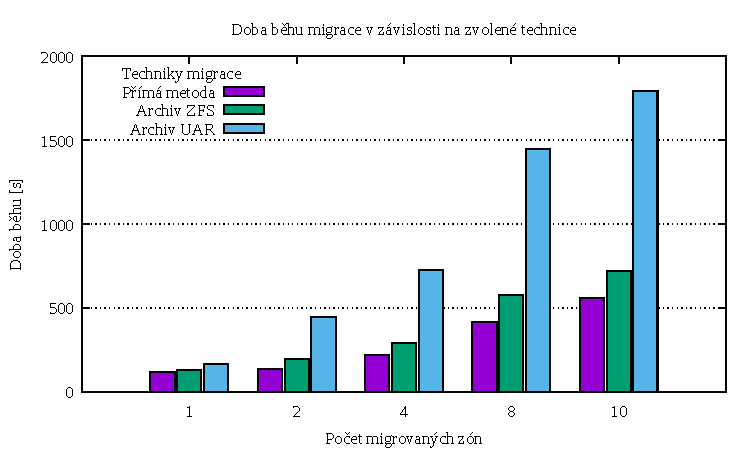
\includegraphics{assets/pdfs/measurement_migration.pdf}
  \caption{Doba běhu vytváření zón v~závislosti na jejich počtu a použité technice}
\end{figure}

Z~provedeného měření je možné vypozorovat, že technika klonování zón je jednoznačně nejrychlejším způsobem vytváření zón. Časy
pro ostatní techniky nejsou tak malé, protože tyto způsoby instalace zahrnují vytváření archivů a přenosy velkých objemů dat
po síti. Velikost jedné neglobální zóny v~průběhu testování byla přibližně 1,5GB. Pokud se má po síti přenášet několik takových
zón najednou, je nutné přenést opravdu velké množství dat. Paralelní instalace zón pomocí těchto technik klade velké nároky na
propustnost sítě i pevných disků. Z~výše uvedeného měření plyne, že technika klonování je v~rámci měřených způsobů nejrychlejší.
Tato technika nešetří pouze čas instalace, ale také diskové místo.
\subsection{Techniky migrace zón}
\label{chapter:measurement:migration}
Druhé měření se zabývá různými technikami způsobu migrace zón a~měří dobu jejich trvání v~závislosti na počtu migrovaných zón.
Implementovaný nástroj umožňuje přenášet zóny mezi servery pomocí následujících technik:
\begin{itemize}
 \item Přímá migrace,
 \item Migrace pomocí ZFS archivu,
 \item Migrace pomocí UAR archivu.
\end{itemize}
První technika využívá k~migraci přímo příkazy souborového systému ZFS a~umožňuje přenášet souborový systém bez nutnosti jeho dočasného
uložení. Migrace pomocí ZFS archivu je podobná přímé technice, ale v~průběhu migrace se zdrojový souborový systém uloží do archivu,
který je následně přenesen na cílový server. V~případě poslední techniky je použitý archiv typu UAR, který je standardním způsobem zálohování
v~operačním systému Solaris. I~tato technika vyžaduje dočasné uložení vytvořeného archivu. Provedené měření bylo zaměřeno
na porovnání doby trvání migrace v~závislosti na počtu migrovaných zón a~zvolené technice migrace.

Pro účel tohoto měření byly na lokálním serveru \textit{shost} vytvořeny neglobální zóny, které byly vždy přesouvány na vzdálený
server \textit{shost1}. Migrace byla několikrát opakována pro každou zmíněnou techniku a~počet migrovaných zón. Výsledná
doba běhu byla v~rámci opakování se stejnými hodnotami parametrů zprůměrována. Stejně jako v~minulém měření bylo přenášeno maximálně
deset neglobálních zón najednou. Naměřené hodnoty doby běhu pro různé počty migrovaných zón a~různé techniky migrace je možné
pozorovat v~tabulce \ref{table:measuremet:migration}. Graficky jsou tyto hodnoty znázorněny v~grafu \ref{graph:measuremet:migration}.
\begin{table}
  \centering
  \label{table:measuremet:migration}
  \caption{Doba běhu migrace zón v~závislosti na použité metodě}
  \begin{tabular}{ l | c c c c c c}
   Počet zón & 1 & 2 & 4 & 8 & 10 &   \\ \hline
   Přímá technika [s] & 118.3 & 134.6 & 220.2 & 420.1 & 561.2 & \\
   Technika ZFS [s] & 133.5 & 196.1 & 291.5 & 580 & 723.7 & \\
   Technika UAR [s] & 167.8 & 449.7 & 729.5 & 1448.3 & 1793.6 & \\
  \end{tabular}
\end{table}

\begin{figure}
  \centering
  \label{graph:measuremet:migration}
  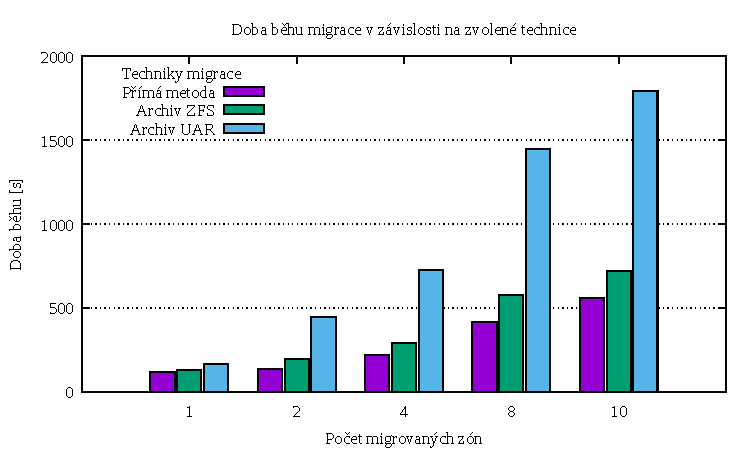
\includegraphics{assets/pdfs/measurement_migration.pdf}
  \caption{Doba běhu migrace zón v~závislosti na použité metodě}
\end{figure}

Z~měření je možné vypozorovat, že přímá technika migrace přenáší zóny nejrychleji. Tento výsledek se byl očekáván, jelikož tato technika nevyžaduje
dočasné ukládání přenášeného souborového systému. Technika využívající ZFS archivy je pomalejší. Důvodem je hlavně nutnost
dočasného uložení vytvořeného archivu na vzdáleném serveru. Výše zmíněné techniky jsou vykonávány paralelně pro všechny přenášené
zóny. V~případě techniky využívající archivy typu UAR tomu tak není. Jak je patrné z~tabulky \ref{table:measuremet:migration},
naměřené časy této techniky odpovídají sériovému provádění migrací. Tento fakt je způsobem nástrojem \verb|archiveadm(1)|, který
nemůže být současně používán více procesy v~rámci jednoho systému. Z~měření vyplynulo, že nejrychlejší technikou pro migraci zón je
přímá technika.
\section{Závěr testování}
\label{chapter:testing:scenario:conclusion}
V~rámci testování nástroje pro podporu automatické správy virtualizačního kontejneru Solaris Zones byly testovány hlavní scénáře
použití a změřena doba běhu některých funkcí nástroje. Popsaná měření dokazují, že implementovaný nástroj je schopen provádět administrátorské
rutiny pro větší množství neglobálních zón. S~rostoucím počtem těchto zón však roste i celková doba běhu programu. Z~měření je také patrné,
že některé funkce nástroje jsou v~určitých situacích výhodnější než jiné.

Všechny testované scénáře byly prováděny v~rámci definovaného prostředí.
Vybrané scénáře použití by měly pokrývat hlavní funkcionalitu nástroje a~jejich splnění by mělo
vypovídat funkčnosti celého nástroje. Jelikož testování těchto scénářů proběhlo bez chyb a~s~očekávanými výsledky, je možné konstatovat,
že implementovaný nástroj splňuje všechny stanovené požadavky a~obsahuje požadovanou funkcionalitu.



\begin{conclusion}
  % Chapter: Conclusion
% Author: Tomáš Šimáček
\label{chapte:conclusion}
Virtualizace se stala běžnou a možná i nezbytnou součástí dnešního počítačového světa. Teto technika se využívá v~mnoha oblastech
informačních technologií, kde přináší různé benefity. Virtualizace umožňuje společnostem efektivně využívat dostupné 
fyzické prostředky a tím výrazně ušetřit náklady na provoz fyzických zařízení. Tématem této diplomové práce byla virtualizace serverů,
která umožňuje současný běh několika virtuálních počítačů v~rámci jednoho fyzického systému.

Jednou z~technik virtualizace serverů je technologie Solaris Zones, která je součástí operačního systému Solaris vyvíjeného firmou Oracle.
Tato virtualizační technika umožňuje běh mnoha virtualizačních kontejnerů v~rámci jedné instance operačního systému Solaris. Tyto
kontejnery se nazývají zóny a jsou izolovány na úrovni počítačové sítě, souborového systému a spuštěných procesů. Standardně hlavní
operační systém sdílí svoje jádro s~ostatními zónami, ale tato technika umožňuje vytvářet i zóny s~vlastním jádrem.

Cílem teoretické části této diplomové práce bylo tuto virtualizační techniku popsat a porovnat s~ostatními běžně využívanými technikami
virtualizace. Dále se práce zaměřila na popis konfigurace, instalace a základních administrátorských rutin pro správu zón.
Předmětem byly také pokročilé rutiny vyžadují provedení několika kroků, jejichž postupným vykonáváním lze dosáhnout požadovaného výsledku. Z~tohoto
důvodu bylo hlavním cílem práce vytvořit nástroj, který by tyto procesy automatizoval a umožnil je provádět i pro vzdálené zóny.
Hlavním důvodem pro vytvoření tohoto nástroje je fakt, že standardní nástroje pro správu Solaris Zones tuto funkcionalitu neposkytují.
Jelikož Solaris Zones poskytují uživateli pouze rozhraní na příkazové řádce, bylo nutné implementovaný nástroj postavit právě nad tímto
rozhraním a využívat tak standardní nástroje pro správu zón.

Výsledná implementace nástroje se skládá z několika částí. Jednou z nich je modul Solaris Zones, který poskytuje funkcionalitu ostatním
částem nástroje. Jeho architektura se skládá z~několika hierarchicky uspořádaných vrstev. Nejníže v~hierarchii se nachází vrstva,
která umožňuje lokální i vzdálené spouštění nástrojů \textit{zonecfg}, \textit{zoneadm}, \textit{archiveadm} a v~neposlední řadě 
také \textit{zfs}. Ostatní vrstvy modulu využívají těchto příkazů a vytvářejí z~nich sekvence, které reprezentují jednotlivé 
administrátorské rutiny pro vytváření, mazání, zálohu, obnovu a migraci zón. Jednotlivé rutiny jsou implementované jako transakce. V~rámci
transakce je zajištěno, že všechny dočasně vytvořené soubory budou smazány a že všechny provedené změny budou navráceny
do původního stavu v~případě neúspěchu transakce. Takto implementované rutiny jsou poskytovány ostatním částem nástroje pomocí
předem definovaného rozhraní. 

Jelikož v~dnešní době existuje mnoho virtualizačních technik s~podobnými vlastnostmi jako Solaris Zones, byla architektura nástroje
navržena tak, aby se dala v~budoucnu lehce rozšířit o~další moduly. Tuto funkcionalitu zajišťuje v~rámci nástroje knihovna, která
jasně definuje rozhraní jednotlivých modulů. Pomocí tohoto rozhraní knihovna zprostředkovává funkcionalitu modulů klientským 
aplikacím. Ve výsledném nástroji je implementován pouze výše zmíněný modul pro podporu správy Solaris Zones. Tato knihovna také
definuje generickou šablonu, která slouží pro popis konkrétních virtuálních strojů. Výše popsaný modul implementuje rozšíření této
generické šablony, které umožňuje uživateli specifikovat konfiguraci, softwarové vybavení a systémové nastavení zón. Tyto šablony
je možné využít pro vytváření většího množství zón s~danými vlastnostmi.

Ovládání nástroje je zajištěno pomocí uživatelského rozhraní, které je uživateli prezentováno pomocí příkazové řádky. Jednotlivé
příkazy umožňují vyvolat odpovídající funkce modulu pro vytváření, mazání, zálohu, obnovu nebo migraci zón. Uživatel může jednoduše 
specifikovat pro jaké zóny chce danou akci provést. Tyto zóny se mohou nacházet na lokálním i vzdáleném serveru a nástroj
pro každou specifikovanou zónu vykoná konkrétní akci pokud možno paralelně. Uživatelské rozhraní dále implementuje 
systém pro správu vzdálených hostů, který umožňuje dané hosty registrovat a specifikovat parametry připojení. Hromadné akce
poskytované uživatelským rozhraním jsou prováděny právě pro všechny registrované hosty. Jelikož se zónami může manipulovat každý
privilegovaný uživatel, implementuje tato část nástroje také uživatelský žurnál. V~žurnálu jsou udržovány jednotlivé stavy zón, aby
bylo možné poznat, zda v~době nepřítomnosti uživatele nedošlo ke změně stavu zón. Další součástí uživatelského rozhraní je
grafický editor šablon, který uživateli poskytuje možnost interaktivní tvorby a editace šablon. Hlavním smyslem tohoto editoru
je odstínění uživatele od implementačních detailů šablon. Tohoto grafického rozhraní je využito i v~případě interaktivní instalace
zón, která uživateli nabízí možnost specifikace vlastností v~průběhu vytváření zón. 

Implementovaný nástroj umožňuje uživateli jednoduchou správu většího množství zón pomocí automatizovaných rutin pro vytváření,
mazání, zálohu, obnovu a migraci těchto zón. Součástí nástroje jsou šablony, které umožňují přesně specifikovat vlastnosti 
vytvářených zón. Tato funkcionalita se dá dobře využít v~procesu vývoje software pro definici produkčních, testovacích a 
vývojářských prostředí. Implementované uživatelské rozhraní prezentuje uživateli funkce nástroje v~jednoduché a přehledné formě.
Grafické součásti nástroje slouží především pro komfortní vytváření a editaci šablon.

Implementovaný nástroj pro podporu automatické správy virtualizačního
kontejneru Solaris Zones poskytuje očekávanou funkcionalitu a splňuje stanovené požadavky. Tato skutečnost byla ověřena v~rámci testování
tohoto nástroje, které je součástí této diplomové práce. Z těchto důvodů je možné konstatovat, že všechny stanovené cíle této diplomové práce 
byly naplněny. Instalační balík a zdrojové kódy implementovaného nástroje i zdrojové kódy celé diplomové práce jsou dostupné na přiloženém médiu.
\end{conclusion}

\bibliographystyle{csn690}
\bibliography{references}

\appendix

\chapter{Seznam použitých zkratek}
% \printglossaries
\begin{description}
        \item[BIOS] Basic Input Output System
        \item[CLI] Command Line Interface
        \item[DNS] Domain Name System
        \item[EPT] Extended Page Tables
        \item[HLL]  High Level Langugage
        \item[HW]  Hardware
        \item[I/O] Input/Output
        \item[ISA]  Instruction Set Architecture
	\item[IT]  Information Technology
	\item[JSON] JavaScript Object Notation
	\item[NAT]  Network Address Transaltion
	\item[OS]  Operating System
	\item[PC]  Program Counter/Personal Computer
	\item[RVI]  Rapid Virtualization Indexing
	\item[SW]  Software
	\item[SMF] Solaris Management Facility
	\item[SSH] Secure Shell
	\item[TLB] Translation Lookaside Buffer
	\item[YARV] Yet Another Ruby VM
	\item[VM]  Virtual Machine
	\item[VMM] Virtual Machine Monitor
	\item[XML] Extesible Markup Language
	\item[ZFS] Zettabyte File System
\end{description}

\chapter{Obsah přiloženého CD}

%upravte podle skutecnosti

\begin{figure}
	\dirtree{%
		.1 readme.txt\DTcomment{stručný popis obsahu CD}.
		.1 exe\DTcomment{adresář se spustitelnou formou implementace}.
		.1 src.
		.2 impl\DTcomment{zdrojové kódy implementace}.
		.2 thesis\DTcomment{zdrojová forma práce ve formátu \LaTeX{}}.
		.1 text\DTcomment{text práce}.
		.2 thesis.pdf\DTcomment{text práce ve formátu PDF}.
		.2 thesis.ps\DTcomment{text práce ve formátu PS}.
	}
\end{figure}

\chapter{Testování}
  \begin{lstlisting}[basicstyle=\scriptsize\ttfamily, caption={Vytvoření neglobálních zón ze šablony}, float,label={code:test:deployment}]  
# szmgmt_cli deploy -b zdev zdev zdev:shost1 zdev:shost2 -s ~/zdev.json 
Solaris zones deployment from virtual machine specification initialized.
  ---------------------------------------------------------
  Options:
                Boot zones: enable
    Rewrite existing zones: disable
                    Source: specification </export/home/zadmin/zdev.json>
  ---------------------------------------------------------
  Loading virtual machine specification.
  Virtual machine specification loaded.
  ---------------------------------------------------------
  Connecting concurrently to hosts 'localhost, shost1, shost2'.
  Processing zone 'zdev' deployment on host 'localhost'.
  Processing zone 'zdev1' deployment on host 'localhost'.
  Processing zone 'zdev' deployment on host 'shost1'.
  Processing zone 'zdev' deployment on host 'shost2'.
  ---------------------------------------------------------
  Deployment finished.
    Status:
      localhost:
        zdev:  success
        zdev1: success
      shost1:
        zdev:  success
      shost2:
        zdev:  success
\end{lstlisting}

\begin{lstlisting}[basicstyle=\scriptsize\ttfamily, caption={Uživatelské žurnál po změně}, float,label={code:test:journal:change}]  
zadmin@shost:~$ szmgm_cli journal status
Tracked zones:
  ...
  Host shost2
      zweb:shost2
           Zone type: solaris
          Zone state: running
                      MISMATCH - Fresh zone state property is installed.
           Zone path: /system/zones/zweb
                      MISMATCH - Fresh zone UUID mismatch.
Untracked zones:
  Host shost2
      zdev-colne:shost2
          Zone type: solaris
         Zone state: installed
          Zone path: /system/zones/zdev-colne
\end{lstlisting}
\begin{lstlisting}[basicstyle=\scriptsize\ttfamily, caption={Uživatelské žurnál po vytvoření zón}, float,label={code:test:journal}]  
zadmin@shost:~$ szmgm_cli journal status
Tracked zones:
  Host localhost
      zdev1:localhost
           Zone type: solaris
          Zone state: running
           Zone path: /system/zones/zdev1
      zdev:localhost
           Zone type: solaris
          Zone state: running
           Zone path: /system/zones/zdev
  Host shost2
      zdev:shost2
           Zone type: solaris
          Zone state: running                      
           Zone path: /system/zones/zdev
  Host shost1
      zdev:shost1
           Zone type: solaris
          Zone state: running
           Zone path: /system/zones/zdev
\end{lstlisting}
\begin{lstlisting}[basicstyle=\scriptsize\ttfamily, caption={Ověření správného vytvoření zóny}, float,label={code:test:deployment:result}]  
zadmin@shost2:~$ zlogin -C  zdev
[Connected to zone 'zweb' console]
Hostname: solaris
solaris console login: admin
Password:
admin@solaris:~$ ifconfig net0
net0: flags=100001000843<UP,BROADCAST,RUNNING,MULTICAST,IPv4,PHYSRUNNING>
    inet 10.164.85.13 netmask ff000000 broadcast 10.255.255.255
admin@solaris:~$ git --version
git version 1.7.9.2
admin@solaris:~$ hg --version
Mercurial Distributed SCM (version 3.4)
simactom@solaris:~$ profiles
System Administrator
...
\end{lstlisting}

\begin{lstlisting}[basicstyle=\scriptsize\ttfamily, caption={Uživatelský žurnál před migrací}, float,label={code:test:migration:before}]  
zadmin@shost:~/repositories/szmgmt$ bundle exec bin/szmgm_cli journal status
Geting fresh information about zones on all registered hosts...
Tracked zones:
  Host localhost
      zmigr1:localhost
           Zone type: solaris
          Zone state: running
           Zone path: /system/zones/zmigr1
      zmigr:localhost
           Zone type: solaris
          Zone state: running
           Zone path: /system/zones/zmigr                 
  Host shost1
      zmigr3:shost1
           Zone type: solaris
          Zone state: running
           Zone path: /system/zones/zmigr3
      zmigr2:shost1
           Zone type: solaris
          Zone state: running
           Zone path: /system/zones/zmigr2      
\end{lstlisting}

\begin{lstlisting}[basicstyle=\scriptsize\ttfamily, caption={Migrace zón}, float,label={code:test:migration}]  
szmgm_cli migrate -t d zmigr zmigr1 zmigr1:shost1 zmigr1:shost1 -d shost2
Solaris zones migration initialized.
  ---------------------------------------------------------
  Options:
                Boot zones: disable
    Rewrite existing zones: disable
  ---------------------------------------------------------
  Connecting concurrently to hosts 'localhost shost1' to perform migration (direct).
  Processing migration of zone 'zmigr1:localhost' to host shost2. 
    See log '/export/home/zadmin/.szmgmt/log/zmigr1_migration_ph5o7o.log'. 
  Processing migration of zone 'zmigr2:shost1' to host shost2. 
    See log '/export/home/zadmin/.szmgmt/log/zmigr2_migration_uy1frm.log'.
  Processing migration of zone 'zmigr3:shost1' to host shost2. 
    See log '/export/home/zadmin/.szmgmt/log/zmigr3_migration_lhc24y.log'.
  Processing migration of zone 'zmigr:localhost' to host shost2. 
    See log '/export/home/zadmin/.szmgmt/log/zmigr_migration_h2rdat.log'.
  ---------------------------------------------------------
  Migration finished.
    Status:
      localhost:
        zmigr:  success
        zmigr1: success
      shost1:
        zmigr2: success
        zmigr3: success

\end{lstlisting}

\begin{lstlisting}[basicstyle=\scriptsize\ttfamily, caption={Stav zóny na serverech po migraci}, float,label={code:test:migration:list}]  
zadmin@shost:~/repositories/szmgmt$ zoneadm list -vic
  ID NAME     STATUS      PATH                         BRAND      IP    
   0 global   running     /                            solaris    shared

zadmin@shost1:~$ zoneadm list -vic
  ID NAME     STATUS      PATH                         BRAND      IP    
   0 global   running     /                            solaris    shared
   
zadmin@shost2:~$ zoneadm list -vic
  ID NAME     STATUS      PATH                         BRAND      IP    
   0 global   running     /                            solaris    shared
   - zmigr1   installed   /system/zones/zmigr1         solaris    excl  
   - zmigr2   installed   /system/zones/zmigr2         solaris    excl
   - zmigr3   installed   /system/zones/zmigr3         solaris    excl  
   - zmigr    installed   /system/zones/zmigr          solaris    excl  
\end{lstlisting}
\begin{lstlisting}[basicstyle=\scriptsize\ttfamily, caption={Uživatelský žurnál po migraci}, float,label={code:test:migration:after}]  
zadmin@shost:~$ szmgmt_cli journal status
Geting fresh information about zones on all registered hosts...
Tracked zones:  
  Host shost2
      zmigr1:shost2
           Zone type: solaris
          Zone state: installed
           Zone path: /system/zones/zmigr1
      zmigr2:shost2
           Zone type: solaris
          Zone state: installed
           Zone path: /system/zones/zmigr2
      zmigr:shost2
           Zone type: solaris
          Zone state: installed
           Zone path: /system/zones/zmigr  
      zmigr3:shost1
           Zone type: solaris
          Zone state: running
           Zone path: /system/zones/zmigr3
\end{lstlisting}

\begin{lstlisting}[basicstyle=\scriptsize\ttfamily, caption={Vytvoření zálohy zón pomocí UAR}, float,label={code:test:backup}]  
zadmin@shost:~$ szmgmt_cli backup zback:shost2 zback1:shost2 zback2:shost1 zback3:shost1
                -d shost -p /zonepool/backup -t uar
Solaris zones backup initialized.
  ---------------------------------------------------------
  Options:
          Backup directory: /zonepool/backup
          Destination host: shost
  ---------------------------------------------------------
  Connecting concurrently to hosts 'shost2, shost1' to perform backup (UAR).
  Processing zone backup of 'zback2:shost1'. 
    See log '/export/home/zadmin/.szmgmt/log/zback2_backup_syikav.log'.
  Processing zone backup of 'zback:shost2'. 
    See log '/export/home/zadmin/.szmgmt/log/zback_backup_71blh4.log'.
  Processing zone backup of 'zback1:shost2'. 
    See log '/export/home/zadmin/.szmgmt/log/zback1_backup_5rks8b.log'.
  Processing zone backup of 'zback3:shost1'. 
    See log '/export/home/zadmin/.szmgmt/log/zback3_backup_shmtgw.log'.
  ---------------------------------------------------------
  Backup finished.
    Status:
      shost2:
        zback: success
        zback1: success
      shost1:
        zback2: success
        zback3: success
\end{lstlisting}
\begin{lstlisting}[basicstyle=\scriptsize\ttfamily, caption={Obnovení zón ze zálohy typu UAR}, float,label={code:test:recovery}]  
zadmin@shost:~$ szmgmt_cli recover zback:shost2 zback1:shost2 zback2:shost1 zback3:shost1 -a \ 
                /zonepool/backup/zback_backup_1525020859.uar \
                /zonepool/backup/zback1_backup_1525020859.uar \
                /zonepool/backup/zback2_backup_1525020859.uar \
                /zonepool/backup/zback3_backup_1525020859.uar
Solaris zones recovery initialized.
  ---------------------------------------------------------
  Options:
                Boot zones: disable
    Rewrite existing zones: disable
  ---------------------------------------------------------
  Connecting concurrently to hosts 'shost2, shost1' to recovery.
  Processing zone 'zback1' recovery on host 'shost2'.
    Source archive: /zonepool/backup/zback1_backup_1525020859.uar.
    See log '/export/home/zadmin/.szmgmt/log/zback1_recovery_vai7x.log'.
  Processing zone 'zback2' recovery on host 'shost1'.
    Source archive: /zonepool/backup/zback2_backup_1525020859.uar.
    See log '/export/home/zadmin/.szmgmt/log/zback2_recovery_lpl0c1.log'.
  Processing zone 'zback' recovery on host 'shost2'.
    Source archive: /zonepool/backup/zback_backup_1525020859.uar.
    See log '/export/home/zadmin/.szmgmt/log/zback_recovery_7ecl60.log'.
  Processing zone 'zback3' recovery on host 'shost1'.
    Source archive: /zonepool/backup/zback3_backup_1525020859.uar.
    See log '/export/home/zadmin/.szmgmt/log/zback3_recovery_7ta1fr.log'.
tes  ---------------------------------------------------------
  Recovery finished.
    Status:
      shost2:
        zback: success
        zback1: success
      shost1:
        zback2: success
        zback3: success
\end{lstlisting}

\end{document}